% A converse to the discrete four-vertex theorem (Tabachnikov's Problem 2).
% Built by scripts/build-paper (pdflatex, deterministic metadata).
\documentclass[11pt]{amsart}

\usepackage[a4paper,margin=1in]{geometry}
\usepackage{amsmath,amssymb,amsthm,mathtools}
\usepackage{microtype}
\usepackage{booktabs}
\usepackage{enumitem}
\usepackage{graphicx}
\usepackage{fancyvrb}
\usepackage{newunicodechar}
\usepackage[colorlinks=true,linkcolor=blue,urlcolor=blue,citecolor=blue]{hyperref}

\pdfinfoomitdate=1
\pdftrailerid{}
\hypersetup{pdftitle={A converse to the discrete four-vertex theorem},
            pdfauthor={Kristoffer Josefsson}}

\tolerance=2000
\emergencystretch=2em

\newtheorem{theorem}{Theorem}[section]
\newtheorem{proposition}[theorem]{Proposition}
\newtheorem{lemma}[theorem]{Lemma}
\newtheorem{corollary}[theorem]{Corollary}
\newtheorem{conjecture}[theorem]{Conjecture}
\theoremstyle{definition}
\newtheorem{definition}[theorem]{Definition}
\newtheorem{example}[theorem]{Example}
\theoremstyle{remark}
\newtheorem{remark}[theorem]{Remark}

% ---------------------------------------------------------------------------
% Notation (draft 2; one meaning per symbol, see Sections 3--5).
%   Z_n indexes vertices P_i and edges [P_i,P_{i+1}] (edge i).
%   kappa_i > 0 curvature at vertex i; r_i = 1/kappa_i (radii only).
%   h_i half-length of edge i, ell_i = 2 h_i; theta_i turning angle;
%   psi_j heading; Gap, Turn closure gap and total turn; D_kappa domain.
%   Frame e_0<e_1<e_2<e_3; readings s_j = kappa_{e_j}, f_j = kappa_{e_j+1};
%   L in R^4 active half-lengths; beta_j block turns; Phi controller;
%   iota slot embedding; cal A active edges, cal Z dormant edges.
%   Four-length system (Sec. 5): readings (1,t,q,l) / (p,q,h,1); Omega the
%   eight walls; split angles alpha_0, alpha_3, gamma_1, gamma_2; S, T pure
%   turns; chi chord equation; eps_1, eps_3 mixed-corner defects;
%   varsigma_a slope; A,B,C,D slope defects; sigma(h,l), phi(p,t,h,l) flag;
%   \hat L(u,v) orthogonal core, Delta = q^2-u^2v^2; rho_1, rho_3 residuals.
%   Peak indices: H global maximum, K highest secondary peak, J repeated max.
% ---------------------------------------------------------------------------
\newcommand{\R}{\mathbb{R}}
\newcommand{\C}{\mathbb{C}}
\newcommand{\Z}{\mathbb{Z}}
\newcommand{\Zn}{\mathbb{Z}/n}
\newcommand{\ii}{\mathrm{i}}
\newcommand{\Gap}{\mathcal{G}}
\newcommand{\Turn}{\mathcal{T}}
\newcommand{\Ctrl}{\Phi}
\newcommand{\DFV}{\operatorname{DFV}}
\newcommand{\Lean}[1]{\texttt{#1}}
% Figures produced separately; a placeholder keeps the build going meanwhile.
\newcommand{\figfile}[2]{\IfFileExists{tabachnikov/figures/#1.pdf}%
  {\includegraphics[width=#2]{tabachnikov/figures/#1.pdf}}%
  {\fbox{figure #1 pending}}}

% Lean source in the appendix: Unicode glyphs mapped for pdflatex.
\providecommand{\gitversion}{unknown}
\newcommand{\leancommit}{\gitversion}
\DefineVerbatimEnvironment{leancode}{Verbatim}{fontsize=\footnotesize}
\newunicodechar{↔}{\ensuremath{\leftrightarrow}}
\newunicodechar{≤}{\ensuremath{\le}}
\newunicodechar{≠}{\ensuremath{\ne}}
\newunicodechar{→}{\ensuremath{\to}}
\newunicodechar{∀}{\ensuremath{\forall}}
\newunicodechar{∃}{\ensuremath{\exists}}
\newunicodechar{¬}{\ensuremath{\neg}}
\newunicodechar{∧}{\ensuremath{\wedge}}
\newunicodechar{∈}{\ensuremath{\in}}
\newunicodechar{ℝ}{\ensuremath{\mathbb{R}}}
\newunicodechar{ℂ}{\ensuremath{\mathbb{C}}}
\newunicodechar{ℕ}{\ensuremath{\mathbb{N}}}
\newunicodechar{κ}{\ensuremath{\kappa}}
\newunicodechar{₀}{\ensuremath{_0}}

\title{A converse to the discrete four-vertex theorem}
\author{Kristoffer Josefsson}
\renewcommand{\datename}{\textit{Version:}}
\date{\texttt{\gitversion}}

\begin{document}

\begin{abstract}
Tabachnikov asked whether every cyclic sequence of positive numbers with at
least two local maxima and two local minima is the sequence of radii of the
circles through consecutive vertex triples of a convex polygon whose
circumcenters lie inside the corresponding vertex angles. We prove this for
every $n\ge 4$, with extrema counted as plateaus. This is the sharp form: by
Dahlberg's discrete four-vertex theorem the condition is also necessary for
nonconstant sequences. Locally near every nonconstant admissible sequence the
polygon can be chosen to depend continuously (indeed $C^1$) on the sequence,
but in general not globally: we give an explicit path of admissible hexagon
data along which no continuous choice of realizing polygons exists. The
existence and continuity results are formalized in Lean~4 with Mathlib.
We also prove the corresponding characterization for circles tangent to three
consecutive supporting lines, using a separate tangential-polygon construction
and Wegner's forward theorem.
\end{abstract}

\maketitle

\section{Introduction}\label{sec:intro}

The four-vertex theorem says that the curvature of a simple closed plane curve
that is not a circle has two local maxima separated by two local minima,
with the values at both minima strictly smaller than those at both maxima.
Gluck~\cite[pp.~295--296]{Gluck1971} proved the converse for continuous
strictly positive curvature. Dahlberg~\cite[Theorem~1.1]{Dahlberg2005}
proved it for smooth signed curvature, provided the two selected maxima
are positive; see \cite{DGPV2007} for the history.

The four-vertex theorem has many discrete versions
\cite{Musin2004,OvsienkoTabachnikov2001,Sedykh1997,Tabachnikov2000,Dahlberg2008,Pak2010}.
In the one studied here the curvature at a vertex of a polygon is the
reciprocal radius of the circle through that vertex and its two neighbours.
Let $P$ be a convex $n$-gon, $n\ge 4$, with vertices $x_1,\dots,x_n$ in cyclic
order. Following Tabachnikov, call $P$ \emph{coherent} if for every $i$ the
center of the circle through $x_{i-1},x_i,x_{i+1}$ lies inside the angle of
$P$ at $x_i$. If $P$ is coherent and no four consecutive vertices lie on a
circle, then the cyclic sequence $r_1,\dots,r_n$ of the radii of these circles
has at least two local maxima and two local minima. This is due to
Musin (see \cite{Tabachnikov2000,Musin2004}); Dahlberg~\cite{Dahlberg2008}
proved a version for simple, locally regular polygons, not necessarily convex,
extending Bilinski's result for convex polygons with obtuse angles~\cite{Bilinski1963}.

In~\cite[Problem~2]{Tabachnikov2008} Tabachnikov posed the converse: a cyclic
sequence $r_1,\dots,r_n$ with at least two local maxima and two local minima
should be the radius sequence of a coherent convex polygon. Pak remarks
that he is not aware of a nontrivial discrete version of the converse
four-vertex theorem \cite[\S21.10, p.~206]{Pak2010}. We prove Tabachnikov's conjecture.

Local extrema are counted as by Dahlberg \cite{Dahlberg2008}. A
\emph{plateau maximum} of a cyclic sequence is a maximal run of equal
consecutive terms, not the whole sequence, whose two outside neighbours are
both strictly smaller. Plateau minima are defined in the same way. Two
extrema are \emph{distinct} if their runs are disjoint.

\begin{theorem}\label{thm:main}
Let $n\ge 4$ and let $r_1,\dots,r_n>0$ be a cyclic sequence with at least two
distinct plateau maxima and two distinct plateau minima. Then there is a
simple, strictly convex, coherent polygon $x_1,\dots,x_n$, listed
counterclockwise, whose circle through $x_{i-1},x_i,x_{i+1}$ has radius $r_i$
for every $i$.
\end{theorem}
% Lean: Gluck.Discrete.tabachnikov_converse_geometric (TabachnikovConverse.lean)

Strict convexity means that, for each edge, all other vertices lie in the
same open half-plane bounded by its supporting line; coherence places each
circumcenter in the interior of the corresponding vertex angle. The same
polygon has signed Menger curvature $1/r_i$.
Moreover, whenever $r_i\ne r_{i+1}$, the four vertices
$x_{i-1},x_i,x_{i+1},x_{i+2}$ do not lie on a common circle, independently of
whether other adjacent radii are equal.
% Lean: Gluck.Discrete.IsCoherentConvexPolygon.signedMengerR2_eq_inv_of_radii,
%       Gluck.Discrete.IsCoherentConvexPolygon.not_concyclic4_of_radius_ne
%       (TabachnikovCharacterization.lean)

Two distinct plateau maxima already force two distinct plateau minima, and
conversely (Lemma~\ref{lem:dfv-plateau}), so either half of the hypothesis
suffices.

\begin{figure}[t]
\centering
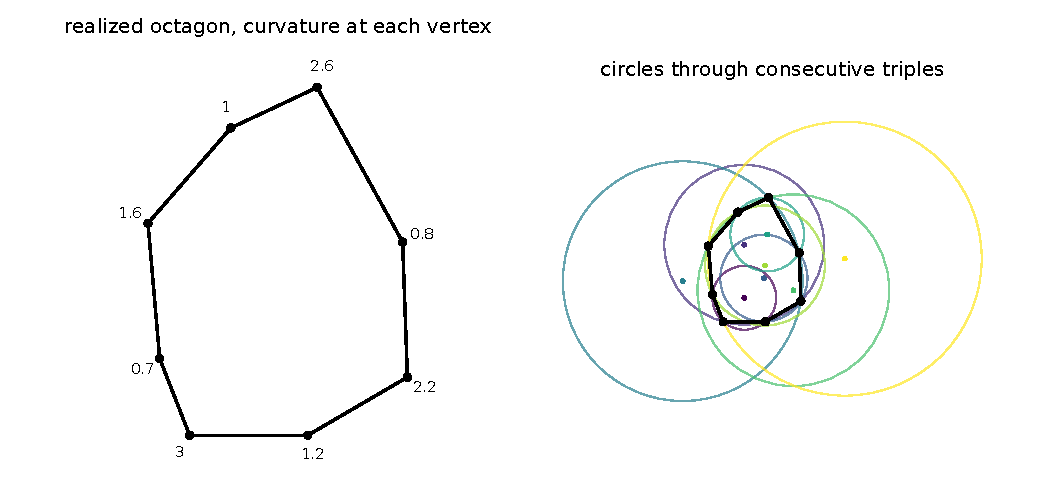
\includegraphics[width=0.7\textwidth]{tabachnikov/figures/example.pdf}
\caption{A coherent convex octagon realizing the curvatures
$(3,1.2,2.2,0.8,2.6,1,1.6,0.7)$, and its eight circles through consecutive
vertex triples, whose centers lie inside the vertex angles. Computed
numerically and checked to double precision.}
\label{fig:example}
\end{figure}

Figure~\ref{fig:example} shows an example. The theorem is sharp:

\begin{corollary}\label{cor:iff}
Let $n\ge4$, and let $r_1,\dots,r_n$ be positive numbers that are not all
equal. Then $r$ is the radius sequence of a coherent convex polygon if and
only if $r$ has two distinct
plateau maxima and two distinct plateau minima.
\end{corollary}

\begin{proof}
One direction is Theorem~\ref{thm:main}. Conversely, a coherent convex
polygon is simple, and its circumcenters lie in the closed vertex sectors,
which is Dahlberg's local regularity \cite{Dahlberg2008}. It is
not inscribed in a circle, since otherwise all the circles through
consecutive triples would coincide and $r$ would be constant. Dahlberg's
discrete four-vertex theorem \cite{Dahlberg2008}, whose extrema
are plateau extrema with distinct runs, gives the two maxima and two minima.
Only its convex case is needed here, since the polygon is strictly convex.
The formalization includes this forward implication and the equivalence.
% Lean: Gluck.Discrete.tabachnikov_radius_characterization
\end{proof}

\begin{remark}[The wording of the problem]\label{rem:wording}
Read with strict extrema, $r_{i-1}<r_i>r_{i+1}$, Tabachnikov's hypothesis
is a special case of Theorem~\ref{thm:main}. Read with weak extrema,
$r_{i-1}\le r_i\ge r_{i+1}$, the statement is false: $r=(2,1,1,1)$ has the
weak local maxima $r_1,r_3$ and minima $r_2,r_4$ but one plateau maximum, so
by Corollary~\ref{cor:iff} it is not a radius sequence. Constant
sequences are excluded by our plateau convention and are realized by regular
$n$-gons.
Tabachnikov's non-concyclicity hypothesis holds for our polygon exactly when
$r_i\ne r_{i+1}$ for all $i$: one implication was just noted, and if
$r_i=r_{i+1}$ in a coherent convex polygon, the circles at $x_i$ and $x_{i+1}$ share the chord
$x_ix_{i+1}$, the radius and the side of their centers, so they coincide.
\end{remark}

It is convenient to work with the curvatures $\kappa_i=1/r_i$. The hypothesis
of Theorem~\ref{thm:main} is then equivalent to a \emph{strict four-vertex
window}: indices $i_1<i_2<i_3<i_4<i_1+n$ and a level $c$ with
\begin{equation}\label{eq:dfv}
  \kappa_{i_2},\ \kappa_{i_4} \;<\; c \;<\; \kappa_{i_1},\ \kappa_{i_3}.
\end{equation}

\subsection*{Organization}
Section~\ref{sec:method} explains the construction informally; the proof
occupies Sections~\ref{sec:setup}--\ref{sec:constructions} and
Appendix~\ref{sec:elimination}. Section~\ref{sec:continuity} shows that the
polygon can be chosen to depend in a $C^1$ way on the data near every
nonconstant admissible sequence (Theorem~\ref{thm:local}), but that a global
continuous choice does not exist, even along a path of admissible
nonconstant hexagon data (Theorem~\ref{thm:hexagon}); the obstruction is the
radius of the smallest enclosing circle. Theorems~\ref{thm:main},
\ref{thm:local} and~\ref{thm:hexagon} are formalized in Lean~4 with Mathlib
\cite{GluckLean}; Appendix~\ref{sec:lean} lists the formal statements.

Tabachnikov also conjectured a converse for the radii of the circles tangent
to three consecutive sides, the discrete four-vertex theorem of
Wegner~\cite{Wegner1994,Tabachnikov2000}; the companion conjecture is also
stated in \cite[Problem~2]{Tabachnikov2008}. Section~\ref{sec:side-tangent} proves this companion converse for inward
circles tangent to the three supporting lines, including their extensions.
It does not use the four-length system of the main theorem.
Section~\ref{sec:discussion} gives a counterexample to the four-vertex theorem
for turning-angle curvature. It also gives a counterexample to the naive
converse for signed Menger curvature and asks what additional hypotheses
are needed for that converse.

\section{The method}\label{sec:method}

We never deform a known polygon. Instead we build the polygon from its edge
lengths. Write $2h_i$ for the length of the edge from vertex $i$ to vertex
$i+1$. A chord of length $2h$ in a circle of curvature $\kappa$ makes the angle
$\arcsin(\kappa h)$ with the tangent at either end, so if the circle through
three consecutive vertices is to have curvature $\kappa_i$, the polygon must
turn at vertex $i$ by
$\theta_i=\arcsin(\kappa_ih_{i-1})+\arcsin(\kappa_ih_i)$. Laying the edges
end to end with these turns, the polygon closes up after one revolution
exactly when three real equations hold: the two coordinates of the closure
gap and the total turn $\sum\theta_i=2\pi$. It therefore suffices to solve
three equations in the $n$ positive half-lengths $h_i$, subject to the bounds
$\kappa_i h_{i-1}<1$ and $\kappa_i h_i<1$. Section~\ref{sec:setup} proves
that every such solution gives a simple, strictly convex, coherent polygon.

\begin{figure}[t]
\centering
\figfile{method}{\textwidth}
\caption{The method, computed for the word
$\mu=(1,\allowbreak\,0.94,\allowbreak\,0.63,\allowbreak\,0.44,\allowbreak\,1.75,\allowbreak\,1.88,\allowbreak\,1.25,\allowbreak\,0.56,\allowbreak\,0.5)$.
(a) The frame of four active edges $e_0,\dots,e_3$ (shaded) and their eight
endpoint readings (black); the other readings (grey) are dormant.
(b) A regular anchor: the dormant edges have length zero, each block of
vertices between two active edges is a single point (open circles), and the
polygon is a quadrilateral. (c) The implicit function theorem opens the
dormant edges to small positive lengths, keeping every prescribed curvature.
(d) Another realization of the same word, for comparison.}
\label{fig:method}
\end{figure}

The main idea is to put all the length on four edges
(Figure~\ref{fig:method}). If every other edge has length zero, the vertices
between two consecutive long edges collapse to one point. The turn at such a
collapsed block involves only the curvatures at its two ends, and the three
equations become three equations in four unknowns that involve only the
eight curvature readings at the ends of the four chosen edges. A positive
solution at which the three equations have full rank is a \emph{regular
anchor}. It is a closed quadrilateral whose corners carry two circles each.
The implicit function theorem then opens every edge of length zero to a small
positive length while keeping all the prescribed curvatures, and the result
is a realization (Section~\ref{sec:anchor}). The same argument, with the
curvatures as parameters, gives the local $C^1$ dependence.

It remains to choose the four edges so that a regular anchor exists. After
removing repeated consecutive curvatures and rescaling, this is a
combinatorial problem about the word $\kappa_1,\dots,\kappa_n$, solved by one
of three explicit constructions, each on a frame of the shape
$(0,\allowbreak\,i-1,\allowbreak\,i,\allowbreak\,n-1)$: the two edges at a peak with curvature $1$ at vertex
$0$ and the two edges at a vertex $i$ further on. The resulting four-length
system depends on five numbers only (Section~\ref{sec:system}).
\begin{description}
\item[(R)] If the maximum of $\kappa$ is attained twice, take the edges at
  the two maxima. An explicit quadrilateral with perpendicular diagonals,
  deformed in two parameters, gives the anchor.
\item[(F)] Otherwise let $0$ be the highest peak other than the global
  maximum $H$. A number $\varphi$ built from the readings next to $0$ and $H$,
  the \emph{forward flag}, decides the construction. If it is nonnegative,
  take the edges at the \emph{first transition}: the first vertex $i$ on the
  way up to $H$ at which the flag of $(\kappa_{i},\kappa_{i+1})$ becomes
  nonnegative.
\item[(N)] If the forward flag and its mirror image, the backward flag, are
  both negative, take the edges at the two peaks $0$ and $H$ and again an
  orthogonal quadrilateral.
\end{description}
Each construction finds a zero by the intermediate value theorem or the
Poincar\'e--Miranda theorem, and proves the rank condition by an explicit
computation (Section~\ref{sec:constructions}).

\section{Development}\label{sec:setup}

Throughout, $n\ge3$, indices of vertices and edges lie in $\Zn$, and
$\kappa=(\kappa_i)_{i\in\Zn}$ is a \emph{profile} of prescribed curvatures.
Edge $i$ joins vertex $i$ to vertex $i+1$; it has length $\ell_i=2h_i$, and
$h_i$ is its \emph{half-length}. For $X,Y,W\in\C$ we write
$[X,Y,W]=\operatorname{Im}\bigl(\overline{(Y-X)}\,(W-X)\bigr)$ for twice the
signed area of the triangle $XYW$, and
\begin{equation}\label{eq:menger}
  M(X,Y,W)=\frac{2\,[X,Y,W]}{|X-Y|\,|Y-W|\,|W-X|}
\end{equation}
for its signed Menger curvature; $|M|$ is the reciprocal circumradius.
% Lean: Gluck.Discrete.crossR2, Gluck.Discrete.signedMengerR2 (TangentChord.lean)
% Lean: Gluck.Discrete.dist_circumcenterR2_mul,
%       Gluck.Discrete.dist_circumcenterR2_eq_inv_abs_signedMenger (TabachnikovConverse.lean)

\begin{definition}\label{def:development}
Let $\kappa\in\R^n$, and let $D_\kappa$ be the open set of $h\in\R^n$ with
$|\kappa_ih_{i-1}|<1$ and $|\kappa_ih_i|<1$ for all $i$. For $h\in D_\kappa$
the \emph{turning angle} at vertex $i$ is
\begin{equation}\label{eq:turning-law}
  \theta_i=\arcsin(\kappa_ih_{i-1})+\arcsin(\kappa_ih_i).
\end{equation}
The \emph{headings} are $\psi_j=\theta_0+\theta_1+\dots+\theta_j$ for
$j\in\mathbb N$ (indices of $\theta$ read mod $n$), the \emph{developed
vertices} are
\begin{equation}\label{eq:vertices}
  P_0=0,\qquad P_k=\sum_{j=0}^{k-1}\ell_j\,e^{\ii\psi_j}\quad(k\in\mathbb N),
\end{equation}
and the \emph{closure gap} and \emph{total turn} are
\begin{equation}\label{eq:gap-turn}
  \Gap(\kappa,h)=P_n\in\C,
  \qquad
  \Turn(\kappa,h)=\sum_{i\in\Zn}\theta_i\in\R.
\end{equation}
For $\kappa>0$, $h$ is \emph{moderate} if $h_i>0$, $\kappa_ih_{i-1}<1$ and
$\kappa_ih_i<1$ for all $i$.
\end{definition}
% Lean: Gluck.Discrete.turningAngle, Gluck.Discrete.heading, Gluck.Discrete.vertexR2,
%       Gluck.Discrete.closureGap, Gluck.Discrete.turningSum (Defs.lean);
%       the Lean functions take full lengths ell = 2h and K = 0.
% Lean: Gluck.Discrete.ModerateArc, Gluck.Discrete.moderateArc_zero_iff (Defs.lean)
% Lean: Gluck.Discrete.contDiffAt_closureGap_lengths,
%       Gluck.Discrete.contDiffAt_turningSum_lengths (DormantOpening.lean)

Figure~\ref{fig:development} illustrates the definition for positive curvature
and moderate half-lengths.

\begin{figure}[htbp]
\centering
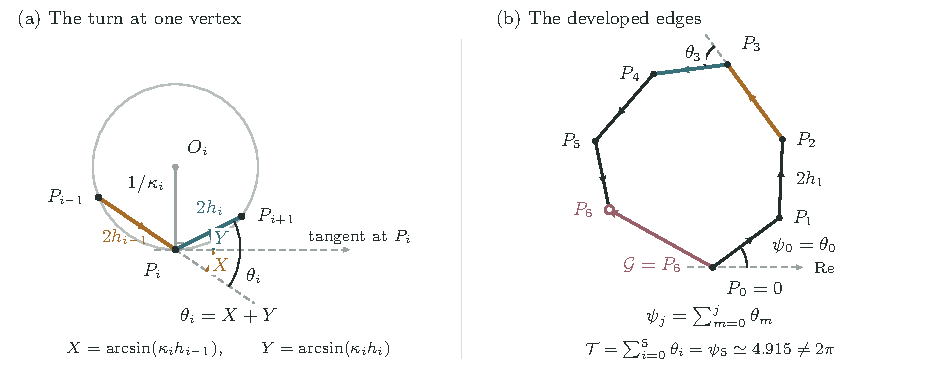
\includegraphics[width=\textwidth]{tabachnikov/figures/development.pdf}
\caption{The quantities in Definition~\ref{def:development}.
(a) The tangent to the circumcircle at $P_i$ splits the exterior turn into
$X$ and $Y$; the incoming edge is continued by a dashed ray.
(b) Edges of length $2h_j$ are placed at headings $\psi_j$.
The highlighted triple $P_2,P_3,P_4$ is the one magnified and rotated in (a),
with $i=3$. The gap arrow runs from $P_0$ to $P_6$; the horizontal reference
shows why the first heading is $\psi_0=\theta_0$.
Here $\Gap\ne0$ and $\Turn\ne2\pi$, so these moderate half-lengths do not
yet give a realization.}
\label{fig:development}
\end{figure}

Both $\Gap$ and $\Turn$ are real-analytic in $(\kappa,h)$ on the open set
where $h\in D_\kappa$, including where some $h_i$ vanish. For moderate $h$
and $\kappa>0$ both arcsines in~\eqref{eq:turning-law} lie in $(0,\pi/2)$, so
$\theta_i\in(0,\pi)$.
% Lean: Gluck.Discrete.turningAngle_pos, Gluck.Discrete.abs_turningAngle_lt_pi (Defs.lean)

\begin{lemma}[Tangent--chord]\label{lem:tangent-chord}
Let $\kappa>0$ and let $h$ be moderate. Then
$M(P_k,P_{k+1},P_{k+2})=\kappa_{k+1}$ for every $k\in\mathbb N$.
\end{lemma}
% Lean: Gluck.Discrete.signedMengerR2_development (TangentChord.lean);
%       Gluck.Discrete.menger_chord_identity (Budget.lean)

\begin{proof}
Put $i=k+1$, $a=\ell_{i-1}$, $b=\ell_i$, $X=\arcsin(\kappa_ia/2)$ and
$Y=\arcsin(\kappa_ib/2)$, so $\theta_i=X+Y$ and $X,Y\in(0,\pi/2)$. The edges
at $P_i$ are $u=ae^{\ii\psi}$ and $w=be^{\ii(\psi+\theta_i)}$ with
$\psi=\psi_{i-1}$. Hence $[P_{i-1},P_i,P_{i+1}]=\operatorname{Im}(\bar
uw)=ab\sin\theta_i$ and, substituting $a=2\sin X/\kappa_i$, $b=2\sin
Y/\kappa_i$,
\[
  \tfrac{\kappa_i^2}{4}|P_{i+1}-P_{i-1}|^2
  =\sin^2\!X+\sin^2\!Y+2\sin X\sin Y\cos(X+Y)=\sin^2(X+Y).
\]
So $\kappa_i|P_{i+1}-P_{i-1}|=2\sin\theta_i$ and
$M=2ab\sin\theta_i/(ab\,|P_{i+1}-P_{i-1}|)=\kappa_i$.
\end{proof}

If $\Gap(\kappa,h)=0$ and $\Turn(\kappa,h)=2\pi$, then $\psi_{j+n}=\psi_j+2\pi$,
so $\ell_{k+n}e^{\ii\psi_{k+n}}=\ell_ke^{\ii\psi_k}$ and, by induction,
$P_{k+n}=P_k$. The development then descends to a closed polygon
$(P_i)_{i\in\Zn}$.
% Lean: Gluck.Discrete.heading_add_n, Gluck.Discrete.vertexR2_add_n,
%       Gluck.Discrete.polygonR2 (Defs.lean)

\begin{definition}\label{def:realization}
Let $\kappa\in\R^n$ be positive. Half-lengths $h$ \emph{realize} $\kappa$ if
$h$ is moderate, $\Gap(\kappa,h)=0$ and $\Turn(\kappa,h)=2\pi$.
\end{definition}
% Lean: Gluck.Discrete.RealizesR2 (Defs.lean); the Lean definition also records
%       IsSimplePolygon, which is automatic by Proposition prop:convex
%       (Gluck.Discrete.isSimplePolygon_of_turningPositive, Convexity.lean).

\begin{proposition}\label{prop:convex}
If $h$ realizes $\kappa$, then $[P_a,P_{a+1},P_c]>0$ whenever
$c\notin\{a,a+1\}$. In particular the polygon $(P_i)_{i\in\Zn}$ is simple and
strictly convex.
\end{proposition}
% Lean: Gluck.Discrete.crossR2_polygonR2_edge_vertex_pos,
%       Gluck.Discrete.support_left_pos, Gluck.Discrete.im_rot_vertex_sub,
%       Gluck.Discrete.isSimplePolygon_of_turningPositive (Convexity.lean)

\begin{proof}
Since every $\theta_i>0$ and $\psi_{j+n}=\psi_j+2\pi$, we have
$\psi_k<\psi_m<\psi_k+2\pi$ for $k<m<k+n$. Fix $k$. For $k\le j$,
\begin{equation}\label{eq:support}
  \operatorname{Im}\bigl(e^{-\ii\psi_k}(P_j-P_k)\bigr)
  =\sum_{m=k}^{j-1}\ell_m\sin(\psi_m-\psi_k),
\end{equation}
and the full sum over $k\le m<k+n$ vanishes. Let $k+1<j<k+n$. If
$\psi_{j-1}-\psi_k\le\pi$, every term in~\eqref{eq:support} is $\ge0$ and the
term $m=k+1$ is $\ell_{k+1}\sin\theta_{k+1}>0$. Otherwise
$\psi_m-\psi_k\in(\pi,2\pi)$ for $j\le m<k+n$, and~\eqref{eq:support} equals
$-\sum_{m=j}^{k+n-1}\ell_m\sin(\psi_m-\psi_k)>0$. Either way
$[P_k,P_{k+1},P_j]>0$. So every vertex off an edge lies in the open left
half-plane of that edge; two non-adjacent edges are separated by the line of
one of them, and consecutive edges meet only in their common vertex.
\end{proof}

A polygon is \emph{coherent} if for every $i$ the triple
$P_{i-1},P_i,P_{i+1}$ is non-collinear and its circumcenter $O_i$ lies in
the open vertex cone
$\{P_i+s(P_{i-1}-P_i)+t(P_{i+1}-P_i):s,t>0\}$.
% Lean: Gluck.Discrete.vertexCone, Gluck.Discrete.CoherentR2 (LocalRegularity.lean)

\begin{proposition}\label{prop:coherent}
If $h$ realizes $\kappa$, the polygon $(P_i)_{i\in\Zn}$ is coherent.
\end{proposition}
% Lean: Gluck.Discrete.coherent_development_moderate,
%       Gluck.Discrete.circumcenterR2_mem_openCone_of_lt (LocalRegularity.lean)

\begin{proof}
Fix $i$, write $u=P_{i-1}-P_i$, $w=P_{i+1}-P_i$, and let $a,b,X,Y$ be as in
the proof of Lemma~\ref{lem:tangent-chord}. Then $\bar uw=-ab\,e^{\ii\theta_i}$,
so $\delta=\operatorname{Im}(\bar uw)=-ab\sin\theta_i\ne0$ and
$\mathcal{C}=\operatorname{Re}(\bar uw)=-ab\cos\theta_i$. The circumcenter is
$O_i=P_i+su+tw$ with
$s=|w|^2(|u|^2-\mathcal C)/(2\delta^2)$ and
$t=|u|^2(|w|^2-\mathcal C)/(2\delta^2)$: indeed
$\langle su+tw,u\rangle=|u|^2(|u|^2|w|^2-\mathcal C^2)/(2\delta^2)=|u|^2/2$,
and likewise for $w$. So $O_i$ lies in the open cone if and only if
$\mathcal C<\min(|u|^2,|w|^2)$. Now
\[
  a^2-\mathcal C=\tfrac{4}{\kappa_i^2}\sin X\bigl(\sin X+\sin Y\cos(X+Y)\bigr)
  =\tfrac{4}{\kappa_i^2}\sin X\sin(X+Y)\cos Y>0,
\]
since $X,Y\in(0,\pi/2)$; the moderate-arc inequalities are used exactly here,
to get $\cos Y>0$. The inequality $b^2-\mathcal C>0$ is symmetric.
\end{proof}

If $\kappa\equiv c>0$, then $h_i=\sin(\pi/n)/c$ realizes $\kappa$: every
$\theta_i=2\pi/n$, and the polygon is the regular $n$-gon.
% Lean: Gluck.Discrete.regularGon_closes (Defs.lean),
%       Gluck.Discrete.realizesR2_const (Convexity.lean)

\subsection{Four-vertex windows and plateau extrema}

\begin{definition}\label{def:dfv}
A profile $\kappa\in\R^n$ has a \emph{strict four-vertex window} at level
$c\in\R$, written $\DFV(\kappa,c)$, if there are integers
$i_1<i_2<i_3<i_4<i_1+n$ satisfying~\eqref{eq:dfv}, indices read mod $n$. A
\emph{plateau maximum run} of $\kappa$ is a cyclic interval
$I=\{a,\dots,a+k\}$ with $k<n-1$ on which $\kappa$ is constant, such that
$\kappa_{a-1}<\kappa_a>\kappa_{a+k+1}$; plateau minimum runs are defined
with the inequalities reversed.
\end{definition}
% Lean: Gluck.Discrete.DFV, Gluck.Discrete.DiscreteFourVertexPos (Converse.lean)
% Lean: Gluck.Discrete.DFV.four_le_period (ConstantRunDFV.lean),
%       Gluck.Discrete.DFV.pos_of_pos (TabachnikovReduction.lean)
% Lean: Gluck.Discrete.PlateauMaxRun, Gluck.Discrete.PlateauMinRun,
%       Gluck.Discrete.IsPlateauLocalMax, Gluck.Discrete.IsPlateauLocalMin
%       (LocalRegularity.lean);
%       Gluck.Discrete.HasTwoPlateauMaxRuns, Gluck.Discrete.HasTwoPlateauMinRuns
%       (TabachnikovReduction.lean)

A window forces $n\ge4$ and, for $\kappa>0$, $c>0$. The runs are the
plateau extrema of Section~\ref{sec:intro}: the strict drops at both ends
force maximality.

\begin{lemma}\label{lem:dfv-plateau}
For $\kappa\in\R^n$ the following are equivalent:
\textup{(a)} $\DFV(\kappa,c)$ for some $c$;
\textup{(b)} $\kappa$ has two disjoint plateau maximum runs;
\textup{(c)} $\kappa$ has two disjoint plateau minimum runs.
\end{lemma}
% Lean: Gluck.Discrete.DFV.plateau_extrema (Converse.lean),
%       Gluck.Discrete.dfv_plateau_extrema (LocalRegularity.lean),
%       Gluck.Discrete.exists_dfv_of_two_plateauMaxRun,
%       Gluck.Discrete.hasTwoPlateauMaxRuns_iff_hasTwoPlateauMinRuns,
%       Gluck.Discrete.discreteFourVertexPos_iff_extrema (TabachnikovReduction.lean)

\begin{proof}
(a)$\Rightarrow$(b),(c). On the integer interval $[i_4-n,i_2]$ the endpoints
are $<c<\kappa_{i_1}$, so a maximum of $\kappa$ on it is attained at an
interior point, and the maximal run of equal values through that point lies
strictly inside the interval. This is a plateau maximum run in
$(i_4-n,i_2)$. The interval $[i_2,i_4]$ gives a disjoint one in
$(i_2,i_4)$. The minimum runs come from $[i_1,i_3]$ and $[i_3,i_1+n]$.

(b)$\Rightarrow$(a). Let $I_1=\{a,\dots,a+k\}$ and $I_2$ be disjoint
plateau maximum runs with values $v_1\le v_2$, and let $a+j$, $0\le j<n$, be
the initial point of $I_2$. Then $j>k$, and $j\ne k+1$, $j\ne n-1$, since
otherwise a strict drop at an end of $I_1$ would give $v_2<v_1$. For $c$
strictly between $\max(\kappa_{a-1},\kappa_{a+k+1})$ and $v_1$, the indices
$a<a+k+1<a+j<a+n-1$ form a window. Apply this to $-\kappa$ for (c).
\end{proof}

Inversion $r\mapsto1/r$ exchanges plateau maxima and minima. So the
hypothesis of Theorem~\ref{thm:main} says exactly that $\kappa=1/r$ has a
strict four-vertex window at some level $c>0$.
% Lean: Gluck.Discrete.discreteFourVertexExtrema_inv (TabachnikovConverse.lean),
%       Gluck.Discrete.tabachnikovProblem2_iff_extrema_form (TabachnikovReduction.lean)

\begin{theorem}\label{thm:dfv-realizes}
Every positive profile with a strict four-vertex window has a realization.
\end{theorem}
% Lean: Gluck.Discrete.realizesR2_of_dfv_fourActive (TabachnikovFourActive.lean);
%       with Proposition prop:regular-polygon:
%       Gluck.Discrete.TabachnikovProblem2 (TabachnikovReduction.lean),
%       Gluck.Discrete.tabachnikovProblem2_all (TabachnikovFourActive.lean)

Theorem~\ref{thm:dfv-realizes} is proved in
Sections~\ref{sec:anchor}--\ref{sec:constructions}.

\begin{proof}[Proof of Theorem~\ref{thm:main}]
Let $\kappa=1/r$ and let $h$ be a realization from
Theorem~\ref{thm:dfv-realizes}, with closed polygon $P$. The polygon is
simple and strictly convex by Proposition~\ref{prop:convex}, and coherent by
Proposition~\ref{prop:coherent}. Lemma~\ref{lem:tangent-chord} and periodicity
give $M(P_{i-1},P_i,P_{i+1})=\kappa_i$, hence the prescribed circumradii.
For the stated local non-concyclicity consequence, if
$P_{i-1},P_i,P_{i+1},P_{i+2}$ lie on a circle with center $O$, then $O$ is the
circumcenter of both non-collinear triples
$P_{i-1},P_i,P_{i+1}$ and $P_i,P_{i+1},P_{i+2}$, so $r_i=|OP_i|=r_{i+1}$.
\end{proof}
% Lean: Gluck.Discrete.tabachnikov_converse_geometric,
%       Gluck.Discrete.signedMengerR2_polygonR2,
%       Gluck.Discrete.eq_circumcenterR2_of_equidist,
%       Gluck.Discrete.vertexCircumradius_eq_of_concyclic (TabachnikovConverse.lean)

\section{Four active edges}\label{sec:anchor}

In this section $\kappa\in\R^n$ is a positive profile. We put all the length
on four edges and give the remaining edges length zero.

\subsection{The controller}

\begin{definition}\label{def:frame}
A \emph{frame} is a choice of edges $0\le e_0<e_1<e_2<e_3\le n-1$. Its
\emph{start} and \emph{finish readings} are
$s_j=\kappa_{e_j}$ and $f_j=\kappa_{e_j+1}$ $(j\in\Z/4)$; the other readings
are \emph{dormant}. On the open set
$U=\{L\in\R^4:|s_jL_j|<1,\ |f_jL_j|<1\}$ put
$a_j=\arcsin(s_jL_j)$, $b_j=\arcsin(f_jL_j)$, define the \emph{block turns}
$\beta_j=b_{j-1}+a_j$ (indices mod $4$) and the \emph{controller}
$\Ctrl=(\Ctrl_1,\Ctrl_2)\colon U\to\C\times\R$,
\begin{equation}\label{eq:controller}
  \Ctrl(L)=\Bigl(L_0+L_1e^{\ii\beta_1}+L_2e^{\ii(\beta_1+\beta_2)}
  +L_3e^{\ii(\beta_1+\beta_2+\beta_3)},\ \
  \beta_0+\beta_1+\beta_2+\beta_3-2\pi\Bigr).
\end{equation}
The \emph{slot embedding} $\iota\colon\R^4\to\R^n$ sets $(\iota L)_{e_j}=L_j$
and $(\iota L)_i=0$ for $i\notin\{e_0,\dots,e_3\}$.
\end{definition}
% Lean: Gluck.Discrete.FourActiveSlots.Frame, .Frame.start, .Frame.finish,
%       .Frame.startArc, .Frame.finishArc, .Frame.turns, .Frame.controller,
%       .Frame.lengths (FourActiveSlotEmbedding.lean).
%       Frame.lengths L returns full lengths 2 L_j; here iota returns half-lengths.

The map $\Ctrl$ is real-analytic on $U$, and $\iota(U)\subset D_\kappa$. In
the development of $\iota L$ the vertices $e_{j-1}+1,\dots,e_j$ of a block
coincide, and only the two outer readings $f_{j-1}$ and $s_j$ contribute to
the turn $\beta_j$ between the active edges $e_{j-1}$ and $e_j$.

\begin{proposition}\label{prop:slot}
For every $L\in U$ \textup{(}no closure hypothesis\textup{)}, with $h=\iota L$,
\begin{equation}\label{eq:slot}
  \Gap(\kappa,h)=2\,e^{\ii\psi_{e_0}(h)}\,\Ctrl_1(L),\qquad
  \Turn(\kappa,h)-2\pi=\Ctrl_2(L).
\end{equation}
\end{proposition}
% Lean: Gluck.Discrete.FourActiveSlots.Frame.closureGap_eq_controller,
%       Gluck.Discrete.FourActiveSlots.Frame.turningSum_eq_controller,
%       Gluck.Discrete.FourActiveSlots.Frame.turningSum_lengths,
%       Gluck.Discrete.FourActiveSlots.Frame.heading_selected,
%       Gluck.Discrete.FourActiveSlots.heading_eq_edge_gap_prefix (FourActiveSlotEmbedding.lean);
%       Gluck.Discrete.sum_gapAngle, Gluck.Discrete.gapAngle (GapCoords.lean)

\begin{proof}
For $h\in D_\kappa$ let
$\gamma_e=\arcsin(\kappa_eh_e)+\arcsin(\kappa_{e+1}h_e)$. Regrouping the
arcsines of~\eqref{eq:turning-law} by edge gives $\Turn=\sum_e\gamma_e$, and
induction on $k$ gives
$\psi_k=\arcsin(\kappa_0h_{n-1})+\sum_{e<k}\gamma_e+\arcsin(\kappa_kh_k)$ for
$0\le k<n$. For $h=\iota L$ we have $\gamma_e=0$ for dormant $e$ and
$\gamma_{e_j}=a_j+b_j$. Hence $\Turn=\sum_j\beta_j$ and
$\psi_{e_j}-\psi_{e_0}=\sum_{i<j}(a_i+b_i)+a_j-a_0=\beta_1+\dots+\beta_j$, so
$\Gap=\sum_j2L_je^{\ii\psi_{e_j}}=2e^{\ii\psi_{e_0}}\Ctrl_1(L)$.
\end{proof}


\subsection{Regular anchors}

\begin{definition}\label{def:anchor}
A \emph{regular anchor} for $\kappa$ is a frame $e_0<\dots<e_3$ together with
$L\in\R^4$ such that
\begin{enumerate}[label=\textup{(A\arabic*)}]
\item\label{it:anchor-pos} $L_j>0$, $s_jL_j<1$ and $f_jL_j<1$ for
  $j=0,\dots,3$;
\item\label{it:anchor-zero} $\Ctrl(L)=0$;
\item\label{it:anchor-reg} the derivative $D\Ctrl(L)\colon\R^4\to\C\times\R$
  is onto.
\end{enumerate}
\end{definition}
% Lean: Gluck.Discrete.RegularFourAnchor (RegularFourAnchor.lean)

\begin{figure}[t]
\centering
\figfile{anchor}{0.4\textwidth}
\caption{The regular anchor of Figure~\ref{fig:method}(b). Only the four
active edges have positive length; the blocks $\{1,2,3\}$ and $\{5,\dots,8\}$
have collapsed to points (open circles). On active edge $e_j$ the two arcs
have curvatures $s_j$ (blue) and $f_j$ (orange), the readings at its two
ends. The turn at each corner is the sum of the two chord angles of the arcs
meeting there, as in~\eqref{eq:controller}.}
\label{fig:anchor}
\end{figure}

Condition~\ref{it:anchor-zero} says that the quadrilateral with half-sides
$L_j$ and exterior angles $\beta_j$ closes with total turn $2\pi$
(Figure~\ref{fig:anchor}), and~\ref{it:anchor-reg} says that the $3\times4$
Jacobian has rank~$3$. The system depends only on $L$ and the eight readings.

\begin{theorem}\label{thm:anchor-realizes}
Let $\kappa^0>0$ admit a regular anchor $(e,\bar L)$. There are an open
neighbourhood $V\subset(0,\infty)^n$ of $\kappa^0$ and a $C^1$ map
$h\colon V\to\R^n$ such that $h(\kappa)$ realizes $\kappa$ for every
$\kappa\in V$. In particular $\kappa^0$ has a realization.
\end{theorem}
% Lean: Gluck.Discrete.RegularFourAnchor.realizesR2 (RegularFourAnchor.lean);
%       Gluck.Discrete.FourActiveSlots.Frame.realizesR2_of_controller_regular,
%       .Frame.fderiv_lengths_at_controller_zero,
%       .Frame.active_surj_of_controller_regular,
%       .Frame.lengths_nonneg_lt_edgeCap (FourActiveSlotEmbedding.lean);
%       Gluck.Discrete.realizesR2_of_regular_dormant_anchor_of_active_surj,
%       Gluck.Discrete.lengthClosureMap_hasStrictFDerivAt_of_nonneg_lt_edgeCap
%       (RegularDormantOpening.lean);
%       Gluck.Discrete.moderateArc_zero_iff_edge (GapCoords.lean);
% Lean (parametric): ContDiffAt.exists_localSection_pos_of_active_surjective
%       (ForMathlib/Analysis/Calculus/ParametricPositiveSection.lean);
%       Gluck.Discrete.RegularFourAnchor.nonempty_localDiscreteRealizationFamily
%       (LocalContinuity.lean)

\begin{proof}
Let $\bar h=\iota\bar L$, let $\mathcal A=\{e_0,\dots,e_3\}$ and
$\mathcal Z=\Zn\setminus\mathcal A$, and let
$G(\kappa,h)=(\Gap(\kappa,h),\Turn(\kappa,h)-2\pi)$, a real-analytic map on the
open set $\{(\kappa,h):h\in D_\kappa\}$. By~\ref{it:anchor-pos}, $\bar L\in U$,
so $\bar h\in D_{\kappa^0}$, and $G(\kappa^0,\bar h)=0$ by~\eqref{eq:slot}
and~\ref{it:anchor-zero}. Write $G_0=D_hG(\kappa^0,\bar h)$.
Differentiating $G(\kappa^0,\iota L)=(g\,\Ctrl_1(L),\Ctrl_2(L))$, with
$g=2e^{\ii\psi_{e_0}\circ\iota}\ne0$, at $\bar L$, the derivative of $g$ drops
out because $\Ctrl_1(\bar L)=0$:
$G_0(\iota v)=(g(\bar L)D\Ctrl_1(\bar L)v,\ D\Ctrl_2(\bar L)v)$. By~\ref{it:anchor-reg},
$G_0$ maps $\R^{\mathcal A}$ onto $\C\times\R$.

So there are $b\in\R^{\mathcal A}$ with $G_0b=-G_0\mathbf 1_{\mathcal Z}$ and a
linear map $N\colon\C\times\R\to\R^{\mathcal A}$ with $G_0N=\mathrm{id}$. Put
$v=\mathbf 1_{\mathcal Z}+b$ and $\widetilde G(\kappa,t,y)=G(\kappa,\bar h+tv+Ny)$ for
$(\kappa,t,y)$ near $(\kappa^0,0,0)$ in $\R^n\times\R\times(\C\times\R)$. Then
$\widetilde G(\kappa^0,0,0)=0$ and $D_y\widetilde G(\kappa^0,0,0)=\mathrm{id}$. The implicit
function theorem gives a neighbourhood $\mathcal N$ of $(\kappa^0,0)$ and a
$C^1$ map $y$ on $\mathcal N$ with $\widetilde G(\kappa,t,y(\kappa,t))=0$. Let
$H(\kappa,t)=\bar h+tv+Ny(\kappa,t)$. Because $N$ takes values in
$\R^{\mathcal A}$, $H_i(\kappa,t)=t$ for $i\in\mathcal Z$. At $(\kappa^0,0)$
the active entries of $H$ are $\bar L_j>0$, and the inequalities
$\kappa_iH_{i-1}<1$, $\kappa_iH_i<1$ hold strictly: they read $s_j\bar L_j<1$
or $f_j\bar L_j<1$ at the ends of an active edge and $0<1$ otherwise. By
continuity there are $t_0>0$ and an open $V\ni\kappa^0$ in $(0,\infty)^n$
such that these strict inequalities and positivity hold at $(\kappa,t_0)$ for
all $\kappa\in V$. Then $h(\kappa)=H(\kappa,t_0)$ is $C^1$, moderate, and
satisfies $\Gap=0$, $\Turn=2\pi$.
\end{proof}

\subsection{Transport of anchors}

\begin{proposition}\label{prop:invariance}
If $\kappa>0$ admits a regular anchor, so do
\textup{(a)} $\lambda\kappa$ for $\lambda>0$;
\textup{(b)} the shift $\kappa(\cdot+a)$ for $a\in\Zn$;
\textup{(c)} the reflection $\kappa(-\,\cdot)$.
\end{proposition}
% Lean: Gluck.Discrete.RegularFourAnchor.scale (RegularFourAnchorTransport.lean);
%       Gluck.Discrete.RegularFourAnchor.comp_add_one, .comp_add, .comp_neg,
%       .of_comp_add, .of_comp_neg, .nonempty_comp_add_iff, .nonempty_comp_neg_iff
%       (RegularFourAnchorCyclic.lean);
%       Gluck.Discrete.FourActiveSlots.Frame.controller_scale_input,
%       .Frame.controller_scale, .Frame.fderiv_controller_scale;
%       Gluck.Discrete.FourActiveSlots.Frame.shiftOneOfPos, .shiftOneOfZero,
%       .Frame.reverse (FourActiveFrameReindex.lean);
%       Gluck.Discrete.FourActiveSlots.slotController_rotate,
%       .slotController_reverse, .Frame.controller_rotate_of_endpoints,
%       .Frame.controller_reverse_of_endpoints (RegularFourAnchorTransport.lean);
%       .Frame.fderiv_controller_rotate_of_endpoints,
%       .Frame.fderiv_controller_reverse_of_endpoints,
%       Gluck.Discrete.RegularFourAnchor.rotateReembed, .reverseReembed
%       (RegularFourAnchorReindex.lean)

\begin{proof}
(a) Keep the frame and take $\bar L/\lambda$; all $\beta_j$ are unchanged and
$\Ctrl^{\lambda\kappa}(L)=(\lambda^{-1}\Ctrl_1^\kappa(\lambda L),\Ctrl_2^\kappa(\lambda L))$.
(b) Take $a=1$. If $e_0\ge1$, the frame $(e_j-1)_j$ has the same readings, and
$\bar L$ works. If $e_0=0$, take the frame $(e_1-1,e_2-1,e_3-1,n-1)$ and
$L'_j=L_{j+1}$ (indices mod $4$). Then $\beta'_j=\beta_{j+1}$ and, since
$\sum_j\beta_j=\Ctrl_2+2\pi$,
\[
  \Ctrl'(L')=\bigl(e^{-\ii\beta_1}\bigl(\Ctrl_1(L)+L_0(e^{\ii\Ctrl_2(L)}-1)\bigr),\
  \Ctrl_2(L)\bigr).
\]
(c) Edge $e$ of $\kappa$ is edge $-e-1$ of $\kappa'=\kappa(-\,\cdot)$,
traversed backwards. Take the frame $e'_j=n-1-e_{3-j}$, with $s'_j=f_{3-j}$,
$f'_j=s_{3-j}$, and $L'_j=L_{3-j}$. Then
$(\beta'_0,\dots,\beta'_3)=(\beta_0,\beta_3,\beta_2,\beta_1)$ and
$\Ctrl'(L')=\bigl(e^{\ii(\beta_1+\beta_2+\beta_3)}\,\overline{\Ctrl_1(L)},\
\Ctrl_2(L)\bigr)$.

In each case $\Ctrl'$ vanishes at the new point, and since $\Ctrl_1$ and
$\Ctrl_2$ vanish there, the derivatives of the prefactors drop out:
$D\Ctrl'$ is $D\Ctrl(\bar L)$ composed with a linear automorphism of
$\C\times\R$ (in~(b), $(z,s)\mapsto(e^{-\ii\bar\beta_1}(z+\ii\bar L_0s),s)$)
and a permutation of $\R^4$. Hence it is onto.
\end{proof}

The controller depends on $\kappa$ only through the eight readings. So if
a frame $e$ for $\mu$ and a frame $e'$ for $\kappa$ have equal readings, a
regular anchor $(e,L)$ for $\mu$ gives the regular anchor $(e',L)$ for
$\kappa$, even if $\mu$ and $\kappa$ have different lengths.
% Lean: Gluck.Discrete.RegularFourAnchor.controller_eq_of_endpoints,
%       Gluck.Discrete.RegularFourAnchor.reembed,
%       Gluck.Discrete.RegularFourAnchor.realizesR2_of_reembed (RegularFourAnchor.lean)

\begin{lemma}\label{lem:constant-run}
Let $\kappa\in\R^{m+1}$, $m\ge1$, with $\kappa_a=\kappa_{a+1}$ for some
$0\le a\le m$, and let $\mu\in\R^m$ be obtained by deleting the entry $a$:
$\mu_i=\kappa_{\tau(i)}$ with $\tau(i)=i$ for $i<a$ and $\tau(i)=i+1$ for
$i\ge a$.
\textup{(i)} If $\DFV(\kappa,c)$, then $\DFV(\mu,c)$.
\textup{(ii)} If $(e,L)$ is a regular anchor for $\mu$, then $(\tau(e),L)$ is
a regular anchor for $\kappa$.
\end{lemma}
% Lean: Gluck.Discrete.ConstantRun.skip, .eraseWord, .collapse, .collapse_mono,
%       .collapse_add_period, .eraseWord_collapse, .eraseWord_dfv, .restoreFrame,
%       .restoreFrame_start, .restoreFrame_finish, .restoreAnchor
%       (ConstantRunAnchorReduction.lean);
%       Gluck.Discrete.DFV.of_monotone_periodic_collapse, Gluck.Discrete.DFV.four_le_period
%       (ConstantRunDFV.lean)

\begin{proof}
(i) The map $\nu\colon\mathbb N\to\mathbb N$ with $\nu(p(m+1)+j)=pm+j$ for
$0\le j\le a$ and $\nu(p(m+1)+j)=pm+j-1$ for $a<j\le m$ is monotone, satisfies
$\nu(i+m+1)=\nu(i)+m$ and $\mu_{\nu(i)}=\kappa_i$. It maps a window
$i_1<\dots<i_4<i_1+m+1$ of $\kappa$ to indices
$\nu(i_1)\le\dots\le\nu(i_4)\le\nu(i_1)+m$, and each inequality is strict
because the two sides carry readings on opposite sides of $c$.
(ii) $\tau$ is strictly increasing, the start readings agree by definition,
and the residues $\tau(e_j)+1$ and $\tau(e_j+1)$ either coincide or are $a$
and $a+1$. So the readings agree.
\end{proof}

A word is \emph{adjacent-unequal} if $\kappa_i\ne\kappa_{i+1}$ for all $i$.

\begin{proposition}\label{prop:reduction}
If every positive adjacent-unequal word with a strict four-vertex window
admits a regular anchor, then every positive profile with a strict four-vertex
window does, and Theorem~\ref{thm:dfv-realizes} holds.
\end{proposition}
% Lean: Gluck.Discrete.ConstantRun.nonempty_regularFourAnchor_of_adjacent_unequal_producer
%       (ConstantRunAnchorReduction.lean);
%       Gluck.Discrete.tabachnikovProblem2_of_adjacent_unequal_regular_anchors
%       (RegularFourAnchorConverse.lean);
%       Gluck.Discrete.nonempty_regularFourAnchor_of_dfv (TabachnikovFourActive.lean)

\begin{proof}
Induct on the length. If $\kappa_a=\kappa_{a+1}$, the shortened word of
Lemma~\ref{lem:constant-run} is positive with a window at the same level, so
it has a regular anchor, which lifts to $\kappa$. Then apply
Theorem~\ref{thm:anchor-realizes}.
\end{proof}

\subsection{Peaks, flags and the case split}\label{ss:split}

For $0<l<1<h$ put
\begin{equation}\label{eq:flag}
  \sigma(h,l)=\sqrt{\frac{1-l^2}{h^2-l^2}},\qquad
  \varphi(p,t,h,l)=\arcsin p+\arcsin\bigl(t\,\sigma(h,l)\bigr)
  -\arcsin\sigma(h,l)-\frac\pi2
\end{equation}
for $0<p<1$ and $0<t\le h$. Here $\sigma\in(0,1)$,
$\sigma^2(h^2-l^2)=1-l^2$ and $h\sigma<1$, because
$(1-h^2\sigma^2)(h^2-l^2)=l^2(h^2-1)>0$; so $t\sigma\le h\sigma<1$ and all
arguments of $\arcsin$ lie in $(0,1)$.
% Lean: Gluck.Discrete.NativeOppositePure.firstPairSigma,
%       Gluck.Discrete.NativeOppositePure.firstPairFlag,
%       Gluck.Discrete.NativeOppositePure.firstPairSigma_data (NativeFirstPairFlag.lean)

A vertex $i$ is a \emph{strict local maximum} if
$\kappa_{i-1}<\kappa_i>\kappa_{i+1}$. For an index $H$, a vertex $K\ne H$ is a
\emph{highest secondary peak relative to $H$} if $K$ is a strict local
maximum and $\kappa_i\le\kappa_K$ for every strict local maximum $i\ne H$.
% Lean: Gluck.Discrete.HighestSecondaryPeak (CurvatureMountainSelection.lean);
%       Gluck.Discrete.IsStrictLocalMax (ZigzagWords.lean)

\begin{lemma}\label{lem:peak}
Let $\kappa$ be adjacent-unequal, let $0$ be a highest secondary peak relative
to $H$, and let $\kappa_0<\kappa_H$. Represent $H$ in $\{0,\dots,n-1\}$.
\begin{enumerate}[label=\textup{(\alph*)}]
\item $H$ is the unique global maximum: $\kappa_i<\kappa_H$ for $i\ne H$.
\item $2\le H\le n-2$, and there is $a$ with $2\le a\le H$,
  $\kappa_{a-1}\le\kappa_0<\kappa_a$, and $\kappa$ strictly increasing on
  $\{a,\dots,H\}$.
\end{enumerate}
\end{lemma}
% Lean (a): not a separate declaration; in the formal case split H is chosen as
%       the global maximum, which supplies the hypothesis
%       (hglobal : ∀ i, i ≠ H → κ i < κ H) of the (N) producer.
% Lean (b): Gluck.Discrete.HighestSecondaryPeak.exists_mountain
%       (CurvatureMountainSelection.lean);
%       .not_isStrictLocalMax, .forward_step, .backward_step, .high_interval,
%       .rising_lt, .falling_lt

\begin{proof}
In an adjacent-unequal word every global maximum is a strict local maximum.

(a) If $G\ne H$ is a global maximum, then $\kappa_G\le\kappa_0<\kappa_H\le\kappa_G$.

(b) Since $\kappa_{\pm1}<\kappa_0<\kappa_H$, $H\notin\{1,n-1\}$. Let $a$ be the
least index in $\{1,\dots,H\}$ with $\kappa_j>\kappa_0$ for $a\le j\le H$; then
$a\ge2$ and $\kappa_{a-1}\le\kappa_0$. If $\kappa_j>\kappa_{j+1}$ for some
$a\le j<H$, the maximum of $\kappa$ on $\{a-1,\dots,j+1\}$ is at least
$\kappa_j>\kappa_0$ and is not attained at the ends, so it is attained at a
strict local maximum $i\ne H$ with $\kappa_i>\kappa_0$, which is impossible.
\end{proof}

Let now $\mu$ be positive and adjacent-unequal with $\mu_0=1$, and let $0$ be
a highest secondary peak relative to $H$ with $\mu_H>1$. By
Lemma~\ref{lem:peak}, $0<\mu_{\pm1}<1$ and $\mu_{H\pm1}<\mu_H$, so the
\emph{forward} and \emph{backward flags}
\[
  \varphi^+=\varphi(\mu_1,\mu_{H-1},\mu_H,\mu_{-1}),\qquad
  \varphi^-=\varphi(\mu_{-1},\mu_{H+1},\mu_H,\mu_1)
\]
are defined. The reflection $\mu'_i=\mu_{-i}$ has $0$ as a highest secondary
peak relative to $-H$, and its forward flag is $\varphi^-$.

\begin{proposition}\label{prop:split}
Every positive adjacent-unequal word with a strict four-vertex window admits a
regular anchor, provided the following hold for all positive adjacent-unequal
words $\mu$ with $\mu_0=1$.
\begin{description}
\item[(R)] If $\mu\le1$ and $\mu_J=1$ for some $J\ne0$, then $\mu$ admits a
  regular anchor.
\item[(F)] If $0$ is a highest secondary peak relative to $H$, $\mu_H>1$ and
  $\varphi^+\ge0$, then $\mu$ admits a regular anchor.
\item[(N)] If $0$ is a highest secondary peak relative to $H$, $\mu_H>1$,
  $\varphi^+<0$ and $\varphi^-<0$, then $\mu$ admits a regular anchor.
\end{description}
\end{proposition}
% Lean: Gluck.Discrete.nonempty_regularFourAnchor_of_adjacent_unequal_dfv,
%       Gluck.Discrete.nonempty_regularFourAnchor_of_repeated_global_maximum,
%       Gluck.Discrete.HighestSecondaryPeak.nonempty_regularFourAnchor,
%       Gluck.Discrete.HighestSecondaryPeak.nonempty_regularFourAnchor_of_forward_terminal,
%       Gluck.Discrete.HighestSecondaryPeak.nonempty_regularFourAnchor_of_backward_terminal,
%       Gluck.Discrete.nonempty_regularFourAnchor_of_normalizedAt
%       (UniversalRegularFourAnchor.lean);
%       Gluck.Discrete.DFV.exists_two_strictLocalMax (N6MonotoneResidue.lean);
%       Gluck.Discrete.exists_highestSecondaryPeak (CurvatureMountainSelection.lean);
%       Gluck.Discrete.normalizedAt, Gluck.Discrete.HighestSecondaryPeak.normalizedAt,
%       Gluck.Discrete.normalizedAt_pos, Gluck.Discrete.normalizedAt_adjacent_ne
%       (FirstPairMountainTransport.lean)

\begin{proof}
Let $\kappa$ be such a word and $H$ a global maximum. For $g\in\Zn$ the word
$\mu^{(g)}_i=\kappa_{i+g}/\kappa_g$ is positive and adjacent-unequal with
$\mu^{(g)}_0=1$, and by Proposition~\ref{prop:invariance} it suffices to find
an anchor for one of them. If the maximum is also attained at $J\ne H$, apply
(R) to $\mu^{(H)}$. Otherwise, by Lemma~\ref{lem:dfv-plateau} $\kappa$ has two
distinct plateau maxima, which are strict local maxima, so there is a
strict local maximum other than $H$; let $K$ be one of largest value. Then
$0$ is a highest secondary peak of $\mu=\mu^{(K)}$ relative to $H-K$, and
$\mu_{H-K}>1$. If $\varphi^+\ge0$, apply (F). If $\varphi^+<0\le\varphi^-$,
apply (F) to the reflection of $\mu$ and use
Proposition~\ref{prop:invariance}(c). If both flags are negative, apply (N).
\end{proof}

Statements (R), (F) and (N) are proved in Section~\ref{sec:constructions}
(Propositions~\ref{prop:R}, \ref{prop:F} and~\ref{prop:N}). Together with
Propositions~\ref{prop:reduction} and~\ref{prop:split} this proves
Theorem~\ref{thm:dfv-realizes}.
% Lean: Gluck.Discrete.realizesR2_of_dfv_fourActive,
%       Gluck.Discrete.tabachnikovProblem2_all (TabachnikovFourActive.lean)

\section{The four-length system}\label{sec:system}

All three constructions use a frame $(0,\,i-1,\,i,\,n-1)$ with $\kappa_0=1$.
Writing $p=\kappa_1$, $t=\kappa_{i-1}$, $q=\kappa_i$, $h=\kappa_{i+1}$ and
$l=\kappa_{-1}$, its readings are
\begin{equation}\label{eq:readings}
  (s_0,s_1,s_2,s_3)=(1,t,q,l),\qquad (f_0,f_1,f_2,f_3)=(p,q,h,1).
\end{equation}
% Lean: Gluck.Discrete.FourActiveSlots.firstPairFrame, firstPairFrame_start,
%       firstPairFrame_finish
In this section $p,t,q,h,l>0$ are arbitrary, and $\Ctrl=\Ctrl_{p,t,q,h,l}$ is
the controller~\eqref{eq:controller} with these readings. Its block turns are
\begin{align*}
  \beta_0&=\arcsin L_3+\arcsin L_0, & \beta_1&=\arcsin(pL_0)+\arcsin(tL_1),\\
  \beta_2&=\arcsin(qL_1)+\arcsin(qL_2), & \beta_3&=\arcsin(hL_2)+\arcsin(lL_3).
\end{align*}
Corners $0$ and $2$ are \emph{pure} (equal readings $1$, resp.\ $q$, on both
sides), corners $1$ and $3$ are \emph{mixed}. Let $\Omega$ be the open set of
$L\in\R^4$ with $L_j>0$ and
\begin{equation}\label{eq:walls}
  L_0<1,\quad pL_0<1,\quad tL_1<1,\quad qL_1<1,\quad qL_2<1,\quad hL_2<1,
  \quad lL_3<1,\quad L_3<1 .
\end{equation}
This is condition~\ref{it:anchor-pos}. So a zero $L\in\Omega$ of $\Ctrl$ at
which $D\Ctrl(L)$ is onto is a regular anchor on every frame with
readings~\eqref{eq:readings}.
% Lean: Gluck.Discrete.NativeOppositePure.lengthTurns,
%       Gluck.Discrete.NativeOppositePure.nativeLengthController,
%       Gluck.Discrete.FourActiveSlots.Frame.controller_eq_nativeLengthController,
%       Gluck.Discrete.NativeOppositePure.NativeLengthPhysical,
%       Gluck.Discrete.RegularFourAnchor.ofNative

\subsection{Split coordinates}

For $L\in\Omega$ the \emph{split angles}
\[
  \alpha_0=\arcsin L_0,\quad \alpha_3=\arcsin L_3,\quad
  \gamma_1=\arcsin(qL_1),\quad \gamma_2=\arcsin(qL_2)
\]
lie in $(0,\pi/2)$, and $L=(\sin\alpha_0,\sin\gamma_1/q,\sin\gamma_2/q,\sin\alpha_3)$.
The pure turns are $S=\alpha_0+\alpha_3=\beta_0$ and $T=\gamma_1+\gamma_2=\beta_2$,
and the mixed turns are
$\beta_1=\arcsin(p\sin\alpha_0)+\arcsin(\frac tq\sin\gamma_1)$ and
$\beta_3=\arcsin(\frac hq\sin\gamma_2)+\arcsin(l\sin\alpha_3)$. Put
\[
  \chi=\sin S-\frac{\sin T}{q},\qquad
  \varepsilon_1=\alpha_3+\gamma_2+\beta_1-\pi,\qquad
  \varepsilon_3=\alpha_0+\gamma_1+\beta_3-\pi,
\]
so that $\varepsilon_1+\varepsilon_3=\Ctrl_2$. Geometrically, $\chi=0$ says
that the diagonal between the mixed corners is a common chord of the circles
of curvature $1$ and $q$ through the pure corners, and
$\varepsilon_1=\varepsilon_3=0$ says that the turns at the mixed corners are
the inscribed-angle turns of these two circles.
% Lean: Gluck.Discrete.NativeOppositePure.StrictAngles, splitHalfLengths,
%       exists_splitHalfLengths_of_physical, nativeLengthPhysical_splitHalfLengths,
%       nativeLengthController_splitHalfLengths;
%       chord, seamLow (= eps_1), seamHigh (= eps_3), lowTurn, highTurn, turnDefect,
%       seamLow_add_seamHigh

\begin{lemma}[Closure identity]\label{lem:identity}
Let $q\ne0$ and let $\alpha_0,\alpha_3,\gamma_1,\gamma_2,\beta_1,\beta_3$ be
arbitrary real numbers. Define $S,T,\chi,\varepsilon_1,\varepsilon_3$ by the
formulas above, $\tau=\varepsilon_1+\varepsilon_3$, and
$E=\sin\alpha_0+\frac{\sin\gamma_1}qe^{\ii\beta_1}+\frac{\sin\gamma_2}qe^{\ii(\beta_1+T)}
+\sin\alpha_3\,e^{\ii(\beta_1+T+\beta_3)}$. Then
\begin{equation}\label{eq:identity}
  E=e^{-\ii\alpha_3}\Bigl(\sin S-\frac{\sin T}{q}\,e^{\ii\varepsilon_1}\Bigr)
  +\sin\alpha_3\,e^{-\ii S}\bigl(e^{\ii\tau}-1\bigr).
\end{equation}
If $L\in\Omega$ and the six numbers are its split angles and mixed turns, then
$\Ctrl(L)=(E,\tau)$, and $\Ctrl(L)=0$ if and only if
$\chi=\varepsilon_1=\varepsilon_3=0$.
\end{lemma}
% Lean: Gluck.Discrete.NativeOppositePure.nativeHalfClosure_eq, native_zero_iff,
%       seamLow_mem_Ioo_of_strictAngles, native_zero_iff_of_strictAngles

\begin{proof}
We use $\sin x+\sin y\,e^{\pm\ii(x+y)}=\sin(x+y)\,e^{\pm\ii y}$. With
$(x,y)=(\gamma_1,\gamma_2)$ and $\beta_1+\gamma_2=\varepsilon_1-\alpha_3+\pi$,
\[
  \tfrac{e^{\ii\beta_1}}{q}\bigl(\sin\gamma_1+\sin\gamma_2\,e^{\ii T}\bigr)
  =\tfrac{\sin T}{q}e^{\ii(\beta_1+\gamma_2)}
  =-\tfrac{\sin T}{q}\,e^{-\ii\alpha_3}e^{\ii\varepsilon_1}.
\]
Since $\beta_1+T+\beta_3=\tau+2\pi-S$, the last term of $E$ is
$\sin\alpha_3\,e^{-\ii S}+\sin\alpha_3\,e^{-\ii S}(e^{\ii\tau}-1)$, and
$\sin\alpha_0+\sin\alpha_3\,e^{-\ii S}=\sin S\,e^{-\ii\alpha_3}$. Adding up
gives~\eqref{eq:identity}.

For $L\in\Omega$, $(E,\tau)=\Ctrl(L)$ by the definitions. If
$\chi=\varepsilon_1=\varepsilon_3=0$, then $\tau=0$ and $E=e^{-\ii\alpha_3}\chi=0$.
Conversely, if $E=\tau=0$, then $\sin S=\frac{\sin T}{q}e^{\ii\varepsilon_1}$.
Here $\sin T>0$, and $\varepsilon_1\in(-\pi,\pi)$ because
$\alpha_3,\gamma_2\in(0,\pi/2)$ and $\beta_1\in(0,\pi)$. The imaginary part
gives $\varepsilon_1=0$, the real part $\chi=0$, and
$\varepsilon_3=\tau-\varepsilon_1=0$.
\end{proof}

\subsection{Rank}

For $a>0$ and $z\in(0,\pi/2)$ with $a\sin z<1$ let
$\varsigma_a(z)=\frac{d}{dz}\arcsin(a\sin z)=a\cos z/\sqrt{1-a^2\sin^2z}>0$.
Since $a^2\cos^2z-(1-a^2\sin^2z)=a^2-1$,
\begin{equation}\label{eq:slope}
  \varsigma_a(z)<1\ \text{ if } a<1,\qquad
  \varsigma_a(z)>1\ \text{ if } a>1 .
\end{equation}
% Lean: Gluck.Discrete.NativeOppositePure.angleSlope, angleSlope_pos,
%       angleSlope_lt_one, one_lt_angleSlope, hasDerivAt_angleAtom
For $L\in\Omega$ put
\[
  A=1-\varsigma_p(\alpha_0),\quad B=1-\varsigma_l(\alpha_3),\quad
  C=1-\varsigma_{t/q}(\gamma_1),\quad D=1-\varsigma_{h/q}(\gamma_2).
\]
They are the derivatives of the defects $z-\arcsin(a\sin z)$, and $D<1$.

\begin{lemma}\label{lem:rank}
Let $0<p<1$, $0<l<1$, $q\ge1$, $0<t<q$ and $h>0$, and let $L\in\Omega$ with
$\Ctrl(L)=0$. Then $A,B,C\in(0,1)$, $S+T>\pi$ and $\cos S<0$. If $D\Ctrl(L)$
is not onto, then
\begin{equation}\label{eq:minors}
  AD=BC\qquad\text{and}\qquad
  \cos S\,(A+B-AD)+\tfrac{\cos T}{q}\,(A+B-AB)=0 .
\end{equation}
\end{lemma}
% Lean: Gluck.Discrete.NativeOppositePure.incident_minors_vanish_of_not_surjective;
%       angle_sums_gt_pi_of_seamLow_zero, cos_first_sum_neg_of_root, cos_first_sum_neg,
%       pi_div_two_lt_first_sum;
%       fderiv_nativeLengthController_surjective_of_fixedTurn_minor,
%       fderiv_nativeLengthController_surjective_of_fixedHalf_minor,
%       incidentHalfLengths, incidentNativeController,
%       differentiableAt_nativeLengthController_of_physical;
%       closureTargetLinearMap, closureTargetLinearMap_surjective,
%       closureTargetLinearMap_eq_zero_iff, hasFDerivAt_incidentNativeController_of_split,
%       hasFDerivAt_nativeSplitController_of_split;
%       hasFDerivAt_splitController_incident, splitDifferential,
%       splitDifferential_surjective_of_det_ne_zero, hasFDerivAt_incidentSplitController,
%       incidentDifferential, incidentDifferential_surjective_of_det_ne_zero

\begin{proof}
By~\eqref{eq:slope}, $A,B,C\in(0,1)$. By Lemma~\ref{lem:identity},
$\chi=\varepsilon_1=\varepsilon_3=0$. Now $\varepsilon_1=0$ reads
$S+T-\pi=(\alpha_0-\arcsin(p\sin\alpha_0))+(\gamma_1-\arcsin(\frac tq\sin\gamma_1))>0$.
If $S\le\pi/2$, then $0<\pi-T<S\le\pi/2$ gives
$\sin T<\sin S=\sin T/q\le\sin T$. So $S\in(\pi/2,\pi)$.

We use two charts near the split angles of $L$: in chart~I the coordinates are
$(S,\alpha_0,\gamma_1)$ with $T$ fixed ($\alpha_3=S-\alpha_0$,
$\gamma_2=T-\gamma_1$), in chart~II they are $(S,\alpha_0,T)$ with $\gamma_1$
fixed. In each chart, $x\mapsto L(x)=(\sin\alpha_0,\sin\gamma_1/q,\sin\gamma_2/q,\sin\alpha_3)$
is smooth with values in $\Omega$ near $x$, and if
$D(\Ctrl\circ L)(x)=D\Ctrl(L)\circ DL(x)$ is onto, so is $D\Ctrl(L)$. Since
$\chi=\varepsilon_1=\tau=0$ at $x$, differentiating~\eqref{eq:identity} kills
every term with an undifferentiated vanishing factor:
\begin{gather*}
  D(\Ctrl\circ L)=\Lambda\circ D(\chi,\varepsilon_1,\varepsilon_3),\\
  \Lambda(x_0,x_1,x_2)=\Bigl(e^{-\ii\alpha_3}\bigl(x_0-\ii\tfrac{\sin T}{q}x_1\bigr)
  +\ii\sin\alpha_3\,e^{-\ii S}(x_1+x_2),\ x_1+x_2\Bigr).
\end{gather*}
$\Lambda\colon\R^3\to\C\times\R$ is injective (if it vanishes, $x_1+x_2=0$, then
$x_0=x_1=0$), hence bijective. So $D\Ctrl(L)$ is onto as soon as the Jacobian
of $(\chi,\varepsilon_1,\varepsilon_3)$ in either chart is invertible. Since
$\varepsilon_1=S+T-\pi-\operatorname{def}_p(\alpha_0)-\operatorname{def}_{t/q}(\gamma_1)$
and
$\varepsilon_3=S+T-\pi-\operatorname{def}_l(\alpha_3)-\operatorname{def}_{h/q}(\gamma_2)$
with $\operatorname{def}_a(z)=z-\arcsin(a\sin z)$, these Jacobians are
\[
  J_{\mathrm I}=\begin{pmatrix}\cos S&0&0\\ 1&-A&-C\\ 1-B&B&D\end{pmatrix},
  \qquad
  J_{\mathrm{II}}=\begin{pmatrix}\cos S&0&-\frac{\cos T}{q}\\ 1&-A&1\\ 1-B&B&1-D\end{pmatrix},
\]
with $\det J_{\mathrm I}=\cos S\,(BC-AD)$ and
$\det J_{\mathrm{II}}=-\cos S\,(A+B-AD)-\frac{\cos T}{q}(A+B-AB)$. As
$\cos S\ne0$, rank loss forces~\eqref{eq:minors}.
\end{proof}

\begin{corollary}\label{cor:rank}
Under the hypotheses of Lemma~\ref{lem:rank}, $D\Ctrl(L)$ is onto in each of
the following cases:
\textup{(a)} $h>q$;
\textup{(b)} $T\ge\pi/2$;
\textup{(c)} $q=1$.
\end{corollary}
% Lean (a): Gluck.Discrete.NativeOppositePure.fderiv_nativeLengthController_surjective_of_physical
%       (splitControllerMinor, controller_minor_neg, splitControllerMinor_det_neg)
% Lean (b): ...fderiv_nativeLengthController_surjective_of_nonacute_incident
%       (fderiv_incidentSplitController_surjective, incidentDifferential_surjective,
%        fderiv_incidentNativeController_surjective)
% Lean (c): ...fderiv_nativeLengthController_surjective_of_equal_pure

\begin{proof}
(a) By~\eqref{eq:slope}, $D<0$, so $BC>0>AD$.
(b) $A+B-AD=B+A(1-D)>0$, $A+B-AB=A+B(1-A)>0$, $\cos S<0$ and $\cos T\le0$, so
the second expression in~\eqref{eq:minors} is negative.
(c) Now $\sin S=\sin T$ and $S+T>\pi$. If $T<\pi/2$, then $0<\pi-S<T<\pi/2$
gives $\sin S<\sin T$. So $T\ge\pi/2$, and (b) applies.
\end{proof}

The remaining case, $h<q$ and $T<\pi/2$, is only needed at the orthogonal
points of the next subsection, where it is settled by an elimination.

\begin{proposition}\label{prop:acute}
Let $0<p,l<1<q$, $0<t,h<q$, and $0<u,v<1$. If $L=\hat L(u,v)$
\textup{(}see~\eqref{eq:core}\textup{)} lies in $\Omega$, $\Ctrl(L)=0$ and
$T<\pi/2$, then $D\Ctrl(L)$ is onto.
\end{proposition}
% Lean: Gluck.Discrete.NativeOppositePure.fderiv_nativeLengthController_surjective_of_acute_orthogonal

The proof is in Appendix~\ref{sec:elimination}.

\subsection{The orthogonal core}

For $q\ge1$ and $u,v\in[0,1]$ with $uv<q$ put $\Delta=q^2-u^2v^2>0$ and
\begin{equation}\label{eq:core}
  \hat L(u,v)=\Delta^{-1/2}\Bigl(\sqrt{q^2-v^2},\ \sqrt{1-v^2},\
  \sqrt{1-u^2},\ \sqrt{q^2-u^2}\Bigr).
\end{equation}
% Lean: Gluck.Discrete.NativeOppositePure.orderedCoreHalfLengths;
%       Gluck.Discrete.N6TypeAThreeCell.rCoreSideA..D, r_core_side_a_half_at_one ..;
%       Gluck.Discrete.orthogonalDelta; Gluck.Discrete.N6TypeAThreeCell.r_denom_pos_aux
Given $p,t,h,l$, the \emph{residuals} are, where defined,
\begin{align*}
  \rho_1(u,v)&=\arcsin(p\hat L_0)+\arcsin(t\hat L_1)-\arcsin(u\hat L_0)-\arcsin(u\hat L_1),\\
  \rho_3(u,v)&=\arcsin(h\hat L_2)+\arcsin(l\hat L_3)-\arcsin(v\hat L_2)-\arcsin(v\hat L_3).
\end{align*}
% Lean: Gluck.Discrete.N6TypeAThreeCell.rResidualOne, rResidualThree, rResidualMap,
%       r_residual_one_eq_core_sides, r_residual_three_eq_core_sides,
%       continuousOn_rResidualOne_of_denom_pos, continuousOn_rResidualThree_of_denom_pos

\begin{lemma}[Orthogonal core]\label{lem:core}
Let $q\ge1$ and write $\hat L=\hat L(u,v)$.
\begin{enumerate}[label=\textup{(\roman*)}]
\item $\hat L_0^2+(v\hat L_2)^2=\hat L_3^2+(u\hat L_1)^2=(q\hat L_1)^2+(v\hat L_3)^2
  =(q\hat L_2)^2+(u\hat L_0)^2=1$.
\item Let $0<u,v<1$. The points $z_0=2\hat L_0\hat L_3$,
  $z_1=2\ii u\hat L_0\hat L_1$, $z_2=-2q\hat L_1\hat L_2$,
  $z_3=-2\ii v\hat L_2\hat L_3$ form a convex quadrilateral with perpendicular
  diagonals and sides $|z_{j+1}-z_j|=2\hat L_j$, the circle through
  $z_{j-1},z_j,z_{j+1}$ has curvature $k_j$, where $(k_0,\dots,k_3)=(1,u,q,v)$,
  and the exterior angle at $z_j$ is
  $\arcsin(k_j\hat L_{j-1})+\arcsin(k_j\hat L_j)$. The controller with readings
  $(1,u,q,v)$, $(u,q,v,1)$ vanishes at $\hat L$.
\item If $0<u,v<1$, $\hat L\in\Omega$ and $\rho_1(u,v)=\rho_3(u,v)=0$, then
  $\Ctrl(\hat L)=0$.
\item $\hat L(v,u)$ is $\hat L(u,v)$ in reverse order, so $\rho_3(u,v)$ equals
  $\rho_1(v,u)$ computed with $(p,t)$ replaced by $(l,h)$.
\item Let $q>1$ and $0<p,l<1$. Where defined,
  $\rho_1(0,v)=\arcsin(p\hat L_0)+\arcsin(t\hat L_1)$ with $\hat L_0>0$; on the
  face $v=1$, $\hat L_1=0$, $\hat L_0>0$, and $\rho_1(u,1)$ has the sign of
  $p-u$; and at the corner $(1,l)$, $\hat L_0=1$, $\hat L_1=\sigma(q,l)$ and
  $\rho_1(1,l)=\varphi(p,t,q,l)$ if $t\le q$. By \textup{(iv)},
  $\rho_3(u,0)=\arcsin(h\hat L_2)+\arcsin(l\hat L_3)$ with $\hat L_3>0$,
  $\rho_3(1,v)$ has the sign of $l-v$, $\rho_3(1,1)=\arcsin l-\pi/2$, and
  $\rho_3(p,1)=\arcsin l+\arcsin(h\sigma(q,p))-\arcsin\sigma(q,p)-\pi/2$, which
  is $\varphi(l,h,q,p)$ if $h\le q$.
\end{enumerate}
\end{lemma}
% Lean: Gluck.Discrete.NativeOppositePure.coreHalfLengths_sq, coreHalfLengths_pos;
%       Gluck.Discrete.N6TypeAThreeCell.r_core_realization_data,
%       r_core_side_half_diagonal_squares, rCoreHalfDiagonalA..D, r_core_sides_pos;
%       Gluck.Discrete.orthogonalA2_identity (...D2), realizesMenger_fourProfile_of_orthogonal,
%       Gluck.Discrete.orthogonalQuad;
%       Gluck.Discrete.NativeOppositePure.native_zero_of_ordered_r_zero,
%       Gluck.Discrete.NativeOppositePure.rResidualThree_eq_swap;
%       rResidualOne_left_pos, rResidualOne_top_zero_iff, r_corner_eq_firstPairFlag,
%       Gluck.Discrete.N6TypeAThreeCell.r_residual_one_bottom_right_eq,
%       r_residual_one_top_left, r_residual_three_top_left_eq,
%       r_residual_three_right_neg

\begin{proof}
(i) Each sum is $\Delta^{-1}$ times $q^2-v^2+v^2(1-u^2)$,
$q^2-u^2+u^2(1-v^2)$, $q^2(1-v^2)+v^2(q^2-u^2)$ or
$q^2(1-u^2)+u^2(q^2-v^2)$, all equal to $\Delta$.

(ii) Here $\hat L>0$. The $z_j$ lie on the four half-axes in counterclockwise
order, so they form a convex quadrilateral whose diagonals meet at $0$. By
Pythagoras and~(i), $|z_1-z_0|^2=4\hat L_0^2(\hat L_3^2+u^2\hat L_1^2)=4\hat L_0^2$,
and likewise for the other sides. In the triangle $z_{j-1}z_jz_{j+1}$ the
neighbours $z_{j\pm1}$ lie on one axis on opposite sides of $0$ and $z_j$ on
the other axis, so the foot of the altitude from $z_j$ is $0$, strictly
between $z_{j-1}$ and $z_{j+1}$, and both base angles are acute. The area is
$\frac12|z_{j+1}-z_{j-1}|\,|z_j|$, so the circumradius is
$|z_j-z_{j-1}|\,|z_{j+1}-z_j|/(2|z_j|)=1/k_j$ (for $j=1$:
$4\hat L_0\hat L_1/(4u\hat L_0\hat L_1)$). By the law of sines the base angle
at $z_{j+1}$ has sine $\frac{k_j}{2}|z_j-z_{j-1}|=k_j\hat L_{j-1}$, so it equals
$\arcsin(k_j\hat L_{j-1})$; likewise the base angle at $z_{j-1}$ is
$\arcsin(k_j\hat L_j)$. The exterior angle at $z_j$ is $\pi$ minus the
interior angle, that is, the sum of the two base angles. In particular the
moderate-arc inequalities $k_j\hat L_{j-1},k_j\hat L_j<1$ hold. Hence the
turning law~\eqref{eq:turning-law} for the profile $k$ with half-lengths
$\hat L$ returns the exterior angles, which sum to $2\pi$, and the development
reproduces the sides of the quadrilateral up to a rotation, so it closes. By
Proposition~\ref{prop:slot} with $n=4$ and no dormant edges, the controller
vanishes at $\hat L$.

(iii) The pure turns $\beta_0,\beta_2$ of $\Ctrl$ at $\hat L$ are those of
the controller in~(ii), and $\rho_1,\rho_3$ are the differences of the mixed
turns. So $\Ctrl(\hat L)$ is the vanishing controller of~(ii).

(iv) Both claims are immediate from~\eqref{eq:core}, since $\Delta$ is
symmetric.

(v) At $u=0$ the subtracted terms vanish. At $v=1$,
$\hat L=\bigl(a,0,\sqrt{1-u^2}/\sqrt{q^2-u^2},1\bigr)$ with
$a=\sqrt{q^2-1}/\sqrt{q^2-u^2}>0$, so
$\rho_1(u,1)=\arcsin(pa)-\arcsin(ua)$. At $(1,l)$, $\Delta=q^2-l^2$, and the
formula follows from~\eqref{eq:flag}. The rest follows from~(iv) and
$\hat L(1,1)=(1,0,0,1)$.
\end{proof}

\subsection{Crossed signs}

\begin{lemma}\label{lem:crossed}
Let $F,G$ be continuous on $Q=[u_1,u_2]\times[v_1,v_2]$, and suppose:
\begin{enumerate}[label=\textup{(\arabic*)}]
\item $F(u_1,v)>0$ and $G(u,v_1)>0$ for all $u,v$;
\item if $G(u_2,v)=0$ then $F(u_2,v)<0$, and if $F(u,v_2)=0$ then $G(u,v_2)<0$;
\item $G(u_2,v_2)<0$.
\end{enumerate}
Then $F$ and $G$ have a common zero in the interior of $Q$.
\end{lemma}
% Lean: Gluck.Discrete.NativeOppositePure.exists_zero_of_two_crossed_corners;
%       Gluck.Hyperbolic.poincareMiranda_rect, ForMathlib: poincare_miranda
%       (ForMathlib/Analysis/Complex/PoincareMiranda.lean).
%       (Draft 1 used a winding-number variant for the (F) rectangle:
%        Gluck.Discrete.ne_zero_of_crossed_fourArcs, windingNumberC_eq_one_of_crossed_fourArcs,
%        Gluck.Discrete.N6TypeAThreeCell.exists_r_residual_zero.)

\begin{proof}
Let $c_1$ and $c_2$ be the clamps of $\R$ onto $[u_1,u_2]$ and $[v_1,v_2]$,
and $R(u,v)=\bigl(u-c_1(u+F),\,v-c_2(v+G)\bigr)$. Then $R_1\le0$ on $u=u_1$,
$R_1\ge0$ on $u=u_2$, $R_2\le0$ on $v=v_1$ and $R_2\ge0$ on $v=v_2$, so by the
Poincar\'e--Miranda theorem $R(z)=0$ for some $z=(u,v)\in Q$. If $u=u_1$, then
$F(z)\le0$, contradicting~(1); so $u>u_1$, and likewise $v>v_1$. If $u=u_2$,
then $F(z)\ge0$; if also $v=v_2$, then $G(z)\ge0$, contradicting~(3), and if
$v<v_2$, then $G(z)=0$, contradicting~(2). If $v=v_2$ and $u<u_2$, then
$F(z)=0$ and $G(z)\ge0$, contradicting~(2). So $z$ is interior, and there
$F(z)=G(z)=0$.
\end{proof}

\section{Existence of anchors}\label{sec:constructions}

We prove statements (R), (F) and (N) of Proposition~\ref{prop:split}. In
each case $\mu$ is positive and adjacent-unequal with $\mu_0=1$, and we
identify $\Zn$ with $\{0,\dots,n-1\}$.

\subsection{A repeated maximum}

\begin{proposition}[Statement (R)]\label{prop:R}
If $\mu\le1$ and $\mu_J=1$ for some $J\ne0$, then $\mu$ has a regular anchor
on the frame $(0,J-1,J,n-1)$.
\end{proposition}
% Lean: Gluck.Discrete.nonempty_regularFourAnchor_of_repeated_normalized_maximum
%       (RepeatedMaximumAnchor.lean),
%       Gluck.Discrete.repeated_maximum_index_separation,
%       Gluck.Discrete.FourActiveSlots.Frame.nonempty_regularFourAnchor_of_repeated_maximum,
%       Gluck.Discrete.NativeOppositePure.exists_r_zero_of_repeated_maximum,
%       equalPeak_first_residual_pos, equalPeak_first_residual_neg,
%       native_zero_of_repeated_r_zero, repeatedMaximumCore_physical,
%       exists_nativeLength_anchor_of_repeated_maximum

\begin{figure}[t]
\centering
\figfile{construct-R}{0.92\textwidth}
\caption{Construction (R) for
$\mu=(1,\allowbreak\,0.57,\allowbreak\,0.70,\allowbreak\,0.83,\allowbreak\,1,\allowbreak\,0.52,\allowbreak\,0.70,\allowbreak\,0.87)$, whose maximum $1$ is
attained at $0$ and $J=4$. The frame is $(0,J-1,J,n-1)$ and the anchor is an
orthogonal quadrilateral (dashed diagonals; Lemma~\ref{lem:core}). Dormant
readings are grey; the arcs are as in Figure~\ref{fig:anchor}. Bottom row: the anchor, the polygon after
opening the dormant edges, and a zoom on the block $\{1,2,3\}$, which is a
single point in the anchor and now has short dormant edges (orange).}
\label{fig:R}
\end{figure}

\begin{proof}
Adjacent inequality gives $2\le J\le n-2$, so the frame is valid
(Figure~\ref{fig:R}). Its readings are~\eqref{eq:readings} with $q=1$ and
$p=\mu_1$, $t=\mu_{J-1}$, $h=\mu_{J+1}$, $l=\mu_{-1}$, which lie in $(0,1)$
because they are at most $1$ and adjacent to a reading equal to $1$. For
$u,v\in(0,1)$ the orthogonal core with $q=1$ is
$\hat L=(\lambda,\lambda,\lambda',\lambda')$ with
$\lambda=\sqrt{1-v^2}/\sqrt{1-u^2v^2}$ and $\lambda'=\sqrt{1-u^2}/\sqrt{1-u^2v^2}$
in $(0,1)$, and
$\rho_1=\arcsin(p\lambda)+\arcsin(t\lambda)-2\arcsin(u\lambda)$,
$\rho_3=\arcsin(h\lambda')+\arcsin(l\lambda')-2\arcsin(v\lambda')$. Let
$a=\frac12\min(p,t,h,l)$ and $b=\frac12(1+\max(p,t,h,l))$, so
$0<a<p,t,h,l<b<1$. Since $\arcsin$ is increasing, $\rho_1>0$ on $u=a$,
$\rho_1<0$ on $u=b$, $\rho_3>0$ on $v=a$ and $\rho_3<0$ on $v=b$. By the
Poincar\'e--Miranda theorem, applied to $(-\rho_1,-\rho_3)$ on $[a,b]^2$, there
is a common zero $(u,v)\in(0,1)^2$. All entries of $\hat L(u,v)$ and all of
$p,t,h,l$ are less than $1$, so $\hat L\in\Omega$, and $\Ctrl(\hat L)=0$ by
Lemma~\ref{lem:core}(iii). Corollary~\ref{cor:rank}(c) gives the rank.
\end{proof}

\subsection{Forward flag nonnegative}

\begin{proposition}[Statement (F)]\label{prop:F}
Let $0$ be a highest secondary peak relative to $H$, $\mu_H>1$ and
$\varphi^+\ge0$. Then $\mu$ has a regular anchor on a frame $(0,i-1,i,n-1)$
with $2\le i<H$.
\end{proposition}
% Lean: Gluck.Discrete.HighestSecondaryPeak.nonempty_regularFourAnchor_of_forward_terminal
%       (UniversalRegularFourAnchor.lean), reducing to
%       Gluck.Discrete.HighestSecondaryPeak.nonempty_regularFourAnchor_of_rising_terminal
%       (FirstPairAnchorSelection.lean);
%       Gluck.Discrete.nonempty_regularFourAnchor_of_rising_mountain_terminal,
%       Gluck.Discrete.exists_firstPair_transition_on_rising_interval,
%       Gluck.Discrete.firstPairFlag_lt_zero_of_le_one, Gluck.Discrete.natPred_val_residue,
%       Gluck.Discrete.NativeOppositePure.exists_regular_anchor_of_firstPair_transition,
%       Gluck.Discrete.FourActiveSlots.Frame.nonempty_regularFourAnchor_of_firstPair_transition

\begin{figure}[t]
\centering
\figfile{construct-F}{0.92\textwidth}
\caption{Construction (F) for
$\mu=(1,\allowbreak\,0.96,\allowbreak\,0.87,\allowbreak\,0.78,\allowbreak\,1.26,\allowbreak\,1.30,\allowbreak\,0.89,\allowbreak\,0.48)$, with maximum at
$H=5$. The frame $(0,i-1,i,n-1)$ sits at the first transition $i=4$ on the
rising leg towards $H$. Here $t=\mu_3\le p=\mu_1$, so the anchor comes from
the chart used when $pt<1$ and is not orthogonal. Bottom row: the anchor, the polygon after
opening the dormant edges, and a zoom on the block $\{1,2,3\}$, which is a
single point in the anchor and now has short dormant edges (orange).}
\label{fig:F}
\end{figure}

\begin{proof}[Choice of the frame]
Let $p=\mu_1$ and $l=\mu_{-1}$, both in $(0,1)$, and let $a$ be as in
Lemma~\ref{lem:peak}(b). For $a-1\le j\le H-1$ we have
$\mu_j\le\mu_{j+1}$ and $\mu_{j+1}>1$, so $\varphi(p,\mu_j,\mu_{j+1},l)$ is
defined, and it is nonnegative for $j=H-1$. Let $i$ be the least such $j$ with
$\varphi(p,\mu_j,\mu_{j+1},l)\ge0$. For $j=a-1$ the flag is negative: with
$\sigma=\sigma(\mu_a,l)$, $\mu_{a-1}\le1$ gives
$\arcsin(\mu_{a-1}\sigma)\le\arcsin\sigma$, and $\arcsin p<\pi/2$. So
$i\ne a-1$. So $a\le i<H$, and with
\[
  t=\mu_{i-1},\quad q=\mu_i,\quad h=\mu_{i+1}
\]
we have $0<t<q$, $1<q<h$ and
\begin{equation}\label{eq:transition}
  \varphi(p,q,h,l)\ \ge\ 0\ >\ \varphi(p,t,q,l).
\end{equation}
Since $2\le a\le i$ and $i+1\le H\le n-2$, $(0,i-1,i,n-1)$ is a frame with
readings~\eqref{eq:readings} (Figure~\ref{fig:F}). By
Corollary~\ref{cor:rank}(a), every zero of $\Ctrl$ in $\Omega$ is regular.
If $t\le p$, then $pt<1$ and Proposition~\ref{prop:chart} below gives a zero;
if $t>p$, Proposition~\ref{prop:ordered} does.
\end{proof}

\begin{lemma}\label{lem:flag}
Let $0<p<1$, $0<l<1<q<h$, $\sigma=\sigma(h,l)$ and $\varphi(p,q,h,l)\ge0$.
Then
\textup{(a)} $\sigma<p$ and $\sqrt{1-p^2}\sqrt{1-\sigma^2}\le(q-p)\sigma$;
\textup{(b)} $pq>1$;
\textup{(c)} $(1-p^2)(h^2-1)\le(1-l^2)(q-p)^2$.
\end{lemma}
% Lean: Gluck.Discrete.NativeOppositePure.arcsin_flag_guard_and_bound /
%       firstPairFlag_guard_and_bound (a), arcsin_flag_one_lt_mul /
%       firstPairFlag_one_lt_mul (b), firstPairFlag_square_bound (c)

\begin{proof}
(a) As $q\sigma<h\sigma<1$, $\arcsin(q\sigma)<\pi/2$, and the flag gives
$\arcsin\sigma<\arcsin p$. The angle $\pi/2-\arcsin p+\arcsin\sigma$ then lies
in $(0,\pi/2)$ and is at most $\arcsin(q\sigma)$; take sines.
(b) From $\sigma<p$, $\sqrt{1-p^2}\,\sigma<p\sqrt{1-\sigma^2}$, so by~(a)
$p(q-p)\sigma\ge p\sqrt{1-p^2}\sqrt{1-\sigma^2}>(1-p^2)\sigma$.
(c) Square~(a) and multiply by $h^2-l^2$, using $\sigma^2(h^2-l^2)=1-l^2$ and
$(1-\sigma^2)(h^2-l^2)=h^2-1$.
\end{proof}

\subsubsection*{The case $t>p$: an orthogonal core}

\begin{proposition}\label{prop:ordered}
Let $0<p<t<q$, $p<1$, $0<l<1<q<h$, and assume~\eqref{eq:transition}. Then
$\Ctrl$ has a zero in $\Omega$.
\end{proposition}
% Lean: Gluck.Discrete.NativeOppositePure.exists_nativeLength_anchor_of_ordered_firstPair,
%       exists_regular_nativeLength_anchor_of_ordered_firstPair, exists_ordered_r_zero,
%       orderedCoreHalfLengths_physical, native_zero_of_ordered_r_zero,
%       exists_r_residual_zero_of_failure;
%       Gluck.Discrete.N6TypeAThreeCell.critical_hWall_pos, critical_hWall_identity,
%       tWall_margin_identity, hWall_margin_identity, r_t_wall_pos_on_rectangle,
%       r_h_wall_pos_on_rectangle, r_actual_t_sideB_wall_lt_one,
%       r_actual_h_sideC_wall_lt_one, r_residual_one_left_pos,
%       r_residual_three_bottom_pos
%       (Lean works on [p,1]x[l,1] with the winding-number lemma; the enlarged
%        rectangle below lets the clamp lemma replace it.)

\begin{proof}
Put $\bar p=\sqrt{1-p^2}$ and $a_*=\sqrt{(h^2-1)/(1-l^2)}$. Since $q>1>p$,
Lemma~\ref{lem:flag}(c) says $p+\bar pa_*\le q$. As $\sigma(h,l)<p$ and
$\sigma(h,l)^2(1+a_*^2)=1$, we get $\bar p<pa_*$; also $a_*^2\ge h^2-1$. Hence
$(p+\bar pa_*)^2-h^2\bar p^2-p^2=\bar p^2(a_*^2-h^2)+2p\bar pa_*
>\bar p^2(a_*^2-h^2+2)>0$, that is,
\begin{equation}\label{eq:hbase}
  q^2-h^2+p^2(h^2-1)>0 .
\end{equation}
For $u,v\in[0,1]$ we have the identities
\begin{align*}
  q^2-u^2v^2-t^2(1-v^2)&=q^2-t^2+v^2(t^2-u^2),\\
  q^2-u^2v^2-h^2(1-u^2)&=\bigl(q^2-h^2+p^2(h^2-1)\bigr)+(u^2-p^2)(h^2-v^2)+p^2(1-v^2).
\end{align*}
The first is positive (if $u>t$ it is at least $q^2-u^2$), so
$t\hat L_1<1$ on $[0,1]^2$. By~\eqref{eq:hbase} there is $p'\in(0,p)$ with
$(p^2-p'^2)h^2<q^2-h^2+p^2(h^2-1)$, and then the second is positive for
$u\ge p'$, so $h\hat L_2<1$ on $[p',1]\times[0,1]$.

Fix $l'\in(0,l)$ and apply Lemma~\ref{lem:crossed} to $F=\rho_1$, $G=\rho_3$
on $Q=[p',1]\times[l',1]$. Both are continuous on $Q$, since all arguments of
$\arcsin$ lie in $[0,1]$ by Lemma~\ref{lem:core}(i) and the two walls just
proved. On $u=p'$,
$\rho_1=(\arcsin(p\hat L_0)-\arcsin(p'\hat L_0))+(\arcsin(t\hat L_1)-\arcsin(p'\hat L_1))>0$
since $\hat L_0>0$ and $p'<p<t$. On $v=l'$, likewise $\rho_3>0$ since
$\hat L_3>0$ and $l'<l<h$. By Lemma~\ref{lem:core}(v), $\rho_3(1,v)=0$ only
for $v=l$, where $\rho_1(1,l)=\varphi(p,t,q,l)<0$ by~\eqref{eq:transition};
$\rho_1(u,1)=0$ only for $u=p$, where $\rho_3(p,1)<0$ by
Lemma~\ref{lem:topleft}; and $\rho_3(1,1)=\arcsin l-\pi/2<0$. So there is a
common zero $(u,v)$ in the interior of $Q$. There $\hat L>0$,
$\hat L_0,\hat L_3,q\hat L_1,q\hat L_2<1$ by Lemma~\ref{lem:core}(i), hence
$p\hat L_0,l\hat L_3<1$, and $t\hat L_1,h\hat L_2<1$ were shown above. So
$\hat L\in\Omega$ and $\Ctrl(\hat L)=0$ by Lemma~\ref{lem:core}(iii).
\end{proof}

\begin{lemma}\label{lem:topleft}
Under the hypotheses of Proposition~\ref{prop:ordered}, with
$\sigma_p=\sigma(q,p)$, we have $h\sigma_p<1$ and
$\rho_3(p,1)=\arcsin l+\arcsin(h\sigma_p)-\arcsin\sigma_p-\pi/2<0$.
\end{lemma}
% Lean: Gluck.Discrete.N6TypeAThreeCell.r_corner_residual_neg_of_failure,
%       strictMonoOn_arcsin_mul_sub_arcsin, r_corner_residual_neg_of_mul_le_one,
%       r_corner_residual_eq_zero_at_threshold, r_corner_threshold_lt_inv,
%       r_corner_residual_neg_of_one_lt_mul

\begin{proof}
The function $g(x)=\arcsin(hx)-\arcsin x$ is strictly increasing on
$[0,1/h]$, because $h/\sqrt{1-h^2x^2}>1/\sqrt{1-x^2}$. By~\eqref{eq:hbase},
$h^2\sigma_p^2(q^2-p^2)=h^2(1-p^2)<q^2-p^2$, so $\sigma_p<1/h$. If $hl\le1$,
then $g(\sigma_p)<g(1/h)=\frac\pi2-\arcsin\frac1h\le\frac\pi2-\arcsin l$. If
$hl>1$, put $d_0=h^2+1-2hl>0$ and $x_0=\sqrt{(1-l^2)/d_0}$. Then
$d_0(1-h^2x_0^2)=(hl-1)^2$ and $d_0(1-x_0^2)=(h-l)^2$, so $x_0<1/h$ and
$\cos g(x_0)=\bigl((hl-1)(h-l)+h(1-l^2)\bigr)/d_0=l$, that is,
$g(x_0)=\frac\pi2-\arcsin l$. Finally $\sigma_p<x_0$: using
$(1-l^2)a_*^2=h^2-1$,
\[
  (1-l^2)\bigl((p+\bar pa_*)^2-p^2\bigr)-\bar p^2d_0=2(1-l^2)p\bar pa_*+2\bar p^2(hl-1)>0,
\]
and $(p+\bar pa_*)^2\le q^2$ gives $\bar p^2d_0<(1-l^2)(q^2-p^2)$, that is,
$\sigma_p^2<x_0^2$.
\end{proof}

\subsubsection*{The case $pt<1$: a chart}

\begin{proposition}\label{prop:chart}
Let $0<p<1$, $0<l<1<q<h$, $t>0$, $pt<1$ and $\varphi(p,q,h,l)\ge0$. Then
$\Ctrl$ has a zero in $\Omega$.
\end{proposition}
% Lean: Gluck.Discrete.NativeOppositePure.exists_native_zero_of_firstPairFlag_of_product_lt_one,
%       exists_regular_anchor_of_firstPairFlag, exists_regular_anchor_of_firstPairFlag_of_le;
%       interiorD (= X), interiorN (= Y), interiorDelta, interiorBeta, interiorHigh,
%       InteriorPhysical, isOpen_interiorPhysical, continuousOn_interiorHigh,
%       interior_seamLow, chord_eliminated, interior_chord, strictAngles_of_interiorPhysical

By Lemma~\ref{lem:flag}(b), $pq>1>pt$, so $t<q$. The chart solves $\chi=0$
and $\varepsilon_1=0$ for $(\alpha_3,\gamma_2)$ given $(\alpha_0,\gamma_1)$. For
$(\alpha_0,\gamma_1)\in\R^2$ let
$\beta_1=\arcsin(p\sin\alpha_0)+\arcsin(\frac tq\sin\gamma_1)$ and
\[
  X=q\cos(\beta_1-\alpha_0)-\cos\gamma_1,\qquad Y=\sin\gamma_1-q\sin(\beta_1-\alpha_0).
\]
For every $\gamma_2$, putting $\alpha_3=\pi-\gamma_2-\beta_1$ (that is,
$\varepsilon_1=0$) gives $q\chi=X\sin\gamma_2-Y\cos\gamma_2$, by expanding
$\sin(\gamma_2+\beta_1-\alpha_0)$. Where $X>0$ let $\hat\gamma_2=\arctan(Y/X)$
and $\hat\alpha_3=\pi-\hat\gamma_2-\beta_1$, so that $\chi=\varepsilon_1=0$.
Let $\mathcal W$ be the open set where $X>0$, $Y>0$,
$0<\hat\alpha_3<\pi/2$ and $\frac hq\sin\hat\gamma_2<1$, and on $\mathcal W$ let
\[
  \mathcal E(\alpha_0,\gamma_1)=\alpha_0+\gamma_1+\arcsin\bigl(\tfrac hq\sin\hat\gamma_2\bigr)
  +\arcsin(l\sin\hat\alpha_3)-\pi
\]
be the value of $\varepsilon_3$. It is continuous, and by
Lemma~\ref{lem:identity} every zero of $\mathcal E$ in
$\mathcal W\cap(0,\pi/2)^2$ gives the zero
$(\sin\alpha_0,\sin\gamma_1/q,\sin\hat\gamma_2/q,\sin\hat\alpha_3)\in\Omega$ of
$\Ctrl$ (here $\hat\gamma_2\in(0,\pi/2)$, and $t<q$).

\emph{The wall $\alpha_0=\pi/2$.} There
$\beta_1=\arcsin p+\arcsin(\frac tq\sin\gamma_1)$, and for $\gamma_1\in[0,\pi/2]$
\begin{align*}
  X&=p\sqrt{q^2-t^2\sin^2\gamma_1}+t\sqrt{1-p^2}\sin\gamma_1-\cos\gamma_1,\\
  Y&=\sqrt{1-p^2}\sqrt{q^2-t^2\sin^2\gamma_1}+(1-pt)\sin\gamma_1 .
\end{align*}
% Lean: wallD, wallN, wallD_eq_trig, wallN_eq_trig, interiorD_wall, interiorN_wall,
%       interiorDelta_wall, interiorBeta_wall, interiorHigh_wall, wallD_pos, wallN_pos,
%       wallDelta_pos, wall_chord, wallBeta_zero_pos, wallBeta_ne_zero, wallBeta_pos,
%       wallBeta_lt_pi_div_two
So $Y>0$, and $X>0$ because
$p^2(q^2-t^2\sin^2\gamma_1)-\cos^2\gamma_1=(p^2q^2-1)+(1-p^2t^2)\sin^2\gamma_1>0$.
On the wall $\chi=0$ reads $\cos\hat\alpha_3=\sin(\gamma_1+\hat\gamma_2)/q>0$.
At $\gamma_1=0$, $\hat\alpha_3=\pi-\hat\gamma_2-\arcsin p>0$, and
$\hat\alpha_3=0$ would force $q=\sin(\gamma_1+\hat\gamma_2)\le1$; so
$0<\hat\alpha_3<\pi/2$ on the wall. At the corner $\gamma_1=0$ we have
$Y=q\sqrt{1-p^2}$, $X=pq-1$, and with $Z=\sqrt{q^2-2pq+1}$,
$\sin\hat\gamma_2=q\sqrt{1-p^2}/Z$ and $\sin\hat\alpha_3=(q-p)/Z$. For
$x=\frac hq\sin\hat\gamma_2$ and $y=l\sin\hat\alpha_3$,
\begin{align*}
  Z^2(1-x^2-y^2)&=(1-l^2)(q-p)^2-(1-p^2)(h^2-1)\ \ge 0,\\
  (1-l^2)Z^2(1-x^2)&=\bigl[(1-l^2)(q-p)^2-(1-p^2)(h^2-1)\bigr]+l^2(1-p^2)(h^2-1)>0
\end{align*}
by Lemma~\ref{lem:flag}(c). So $x<1$ and $\arcsin x+\arcsin y\le\pi/2$, that is,
\begin{equation}\label{eq:corner}
  (\tfrac\pi2,0)\in\mathcal W\qquad\text{and}\qquad
  \mathcal E(\tfrac\pi2,0)=\arcsin x+\arcsin y-\tfrac\pi2\le0 .
\end{equation}
% Lean: wallN_zero, wallD_zero, sin_wallDelta_zero, sin_wallBeta_zero,
%       wall_initial_hwall, arcsin_add_arcsin_le_half_pi, wall_initial_high_nonpos

\emph{Exit.} Let $f(\gamma_1)=\frac hq\sin\hat\gamma_2(\frac\pi2,\gamma_1)$ and
$g(\gamma_1)=\mathcal E(\frac\pi2,\gamma_1)$ on $[0,\pi/2]$; $g$ is continuous
where $f\le1$, and $f(0)<1$. If $f=1$ somewhere, let $e$ be the first such
point; then $g(e)=e+\arcsin(l\sin\hat\alpha_3)>0$. Otherwise let $e=\pi/2$;
then $g(e)=\arcsin(\frac hq\sin\hat\gamma_2)+\arcsin(l\sin\hat\alpha_3)>0$.
Choose $\gamma_{\mathrm{hi}}<e$ with $g(\gamma_{\mathrm{hi}})>0$. Then
$\{\pi/2\}\times[0,\gamma_{\mathrm{hi}}]\subset\mathcal W$.
% Lean: exists_positive_before_first_wall, exists_wall_positive_endpoint,
%       wall_high_pos_at_hwall, wall_high_pos_at_right,
%       exists_physical_boundary_strip_of_firstPairFlag_of_product_lt_one

\emph{Inward derivative.} At $\gamma_1=0$, $\beta_1=\arcsin(p\sin\alpha_0)$ has
derivative $0$ at $\alpha_0=\pi/2$. There $\partial_{\alpha_0}X=-q\sqrt{1-p^2}$
and $\partial_{\alpha_0}Y=qp$, so
$\partial_{\alpha_0}\hat\gamma_2=q(pX+\sqrt{1-p^2}\,Y)/(X^2+Y^2)>0$,
$\partial_{\alpha_0}\hat\alpha_3=-\partial_{\alpha_0}\hat\gamma_2$, and
$\partial_{\alpha_0}\mathcal E(\frac\pi2,0)
=1+(\varsigma_{h/q}(\hat\gamma_2)-\varsigma_l(\hat\alpha_3))\,\partial_{\alpha_0}\hat\gamma_2>1$
by~\eqref{eq:slope}.
% Lean: hasDerivAt_lowTurn_boundary, hasDerivAt_interiorD_boundary,
%       hasDerivAt_interiorN_boundary, exists_pos_derivative_interiorDelta_boundary,
%       exists_derivative_gt_one_interiorHigh_boundary

\begin{proof}[Proof of Proposition~\ref{prop:chart}]
Since $\{\pi/2\}\times[0,\gamma_{\mathrm{hi}}]$ is compact, the segments
$\{\alpha_0\}\times[0,\gamma_{\mathrm{hi}}]$ lie in $\mathcal W$ and
$\mathcal E(\alpha_0,\gamma_{\mathrm{hi}})>0$ for $\alpha_0$ near $\pi/2$. By
\eqref{eq:corner} and the inward derivative (needed when
$\mathcal E(\frac\pi2,0)=0$), $\mathcal E(\alpha_0,0)<0$ for
$\alpha_0<\pi/2$ near $\pi/2$. For such an $\alpha_0\in(0,\pi/2)$ the
intermediate value theorem gives $\gamma_1\in(0,\gamma_{\mathrm{hi}})$ with
$\mathcal E(\alpha_0,\gamma_1)=0$.
\end{proof}
% Lean: Gluck.Discrete.CompactBoundaryIVT.exists_inward_zero_of_boundary_derivative,
%       exists_inward_zero, eventually_lt_left_of_hasDerivAt_pos,
%       exists_strict_root_of_interior_strip,
%       exists_strict_root_of_firstPairFlag_of_product_lt_one

\subsection{Both flags negative}

\begin{proposition}[Statement (N)]\label{prop:N}
Let $0$ be a highest secondary peak relative to $H$, $\mu_H>1$,
$\varphi^+<0$ and $\varphi^-<0$. Then $\mu$ has a regular anchor on the frame
$(0,H-1,H,n-1)$.
\end{proposition}
% Lean: Gluck.Discrete.HighestSecondaryPeak.nonempty_regularFourAnchor_of_negative_terminals
%       (NegativeCornerAnchorSelection.lean; takes hglobal, supplied by Lemma lem:peak(a));
%       Gluck.Discrete.FourActiveSlots.Frame.nonempty_regularFourAnchor_of_negative_corners,
%       Gluck.Discrete.NativeOppositePure.exists_nativeLength_regular_of_negative_corners,
%       exists_nativeLength_anchor_of_negative_corners, exists_r_zero_of_negative_corners,
%       negativeCornersCore_physical,
%       fderiv_nativeLengthController_surjective_of_incident_orthogonal

\begin{figure}[t]
\centering
\figfile{construct-N}{0.92\textwidth}
\caption{Construction (N) for
$\mu=(1,\allowbreak\,0.96,\allowbreak\,0.81,\allowbreak\,0.67,\allowbreak\,1.04,\allowbreak\,0.75,\allowbreak\,0.83,\allowbreak\,0.92)$: the secondary
peak is $0$ and the maximum is $H=4$, and both flags are negative. The frame
is $(0,H-1,H,n-1)$ and the anchor is an orthogonal quadrilateral (dashed
diagonals; Lemma~\ref{lem:core}). Bottom row: the anchor, the polygon after
opening the dormant edges, and a zoom on the block $\{1,2,3\}$, which is a
single point in the anchor and now has short dormant edges (orange).}
\label{fig:N}
\end{figure}

\begin{proof}
By Lemma~\ref{lem:peak}, $2\le H\le n-2$ and $\mu_{H\pm1}<\mu_H$. The frame
(Figure~\ref{fig:N}) has readings~\eqref{eq:readings} with $i=H$:
$p=\mu_1$, $t=\mu_{H-1}$, $q=\mu_H$, $h=\mu_{H+1}$, $l=\mu_{-1}$, where
$0<p,l<1<q$ and $t,h<q$; moreover $\varphi^+=\varphi(p,t,q,l)$ and
$\varphi^-=\varphi(l,h,q,p)$. Apply Lemma~\ref{lem:crossed} to $F=\rho_1$,
$G=\rho_3$ on $[0,1]^2$; they are continuous there, because all arguments of
$\arcsin$ lie in $[0,1]$ by Lemma~\ref{lem:core}(i). By
Lemma~\ref{lem:core}(v): $\rho_1(0,v)>0$ and $\rho_3(u,0)>0$;
$\rho_3(1,v)=0$ forces $v=l$, where $\rho_1(1,l)=\varphi^+<0$;
$\rho_1(u,1)=0$ forces $u=p$, where $\rho_3(p,1)=\varphi^-<0$; and
$\rho_3(1,1)<0$. So there is a common zero $(u,v)\in(0,1)^2$. By
Lemma~\ref{lem:core}(i), $\hat L_0,\hat L_3,q\hat L_1,q\hat L_2<1$, and with
$p,l<1$ and $t,h<q$ all eight walls hold, so $\hat L\in\Omega$ and
$\Ctrl(\hat L)=0$ by Lemma~\ref{lem:core}(iii). If $T\ge\pi/2$,
Corollary~\ref{cor:rank}(b) gives the rank, and otherwise
Proposition~\ref{prop:acute}.
\end{proof}

\section{Continuity}\label{sec:continuity}

We identify a curvature profile with a vector $\kappa\in\R^n$ and a labelled
polygon with a vector $(P_i)_{i\in\Zn}\in\C^n$, with the product topologies.

\subsection{Local continuity}

\begin{theorem}\label{thm:local}
Let $n\ge4$ and let $\kappa^0\in\R^n$ be positive with a strict four-vertex
window~\eqref{eq:dfv}. There are an open neighbourhood $V$ of $\kappa^0$ and
$C^1$ maps $h\colon V\to\R^n$ and $P\colon V\to\C^n$ such that for every
$\kappa\in V$ the half-lengths $h(\kappa)$ realize $\kappa$ and $P(\kappa)$ is
the polygon developed from them by~\eqref{eq:vertices}, normalized by
$P_0=0$. In particular $P(\kappa)$ is simple, strictly convex and coherent,
with curvature $\kappa_i$ at every vertex.
\end{theorem}
% Lean: Gluck.Discrete.localContinuousRealization_of_dfv
%       (Gluck/Discrete/LocalContinuity.lean).

\begin{proof}
By Propositions~\ref{prop:reduction} and~\ref{prop:split} and
Section~\ref{sec:constructions}, $\kappa^0$ has a regular anchor, and
Theorem~\ref{thm:anchor-realizes} gives $V$ and $h$. The vertices
\eqref{eq:vertices} are real-analytic in $(\kappa,h)$, so $P$ is $C^1$. The
remaining properties are Section~\ref{sec:setup}.
\end{proof}

\subsection{No global continuous choice}

For $0\le s\le1$ consider the hexagon profile
\begin{equation}\label{eq:band}
  \kappa^{s} = (14,\ 11,\ 10+3s,\ 5,\ 7-3s,\ 3).
\end{equation}
Every $\kappa^s$ is positive and nonconstant. A direct check of all
quadruples of indices shows that the levels $c$ of strict four-vertex windows
of $\kappa^s$ form the set
\[
  (5,\,7-3s)\ \cup\ (11,\,10+3s),
\]
with an empty interval when the endpoints are reversed. The lower band is
nonempty for $s<2/3$ (window indices $0,3,4,5$), the upper band for $s>1/3$
(indices $0,1,2,5$). Hence every $\kappa^s$ is admissible and, by
Theorem~\ref{thm:main}, realized by a coherent convex hexagon.
% Lean: bandProfile_dfv_iff, bandProfile_admissible,
%       bandProfile_pointwise_realizable (Gluck/Discrete/GlobalContinuity)

\begin{figure}[t]
\centering
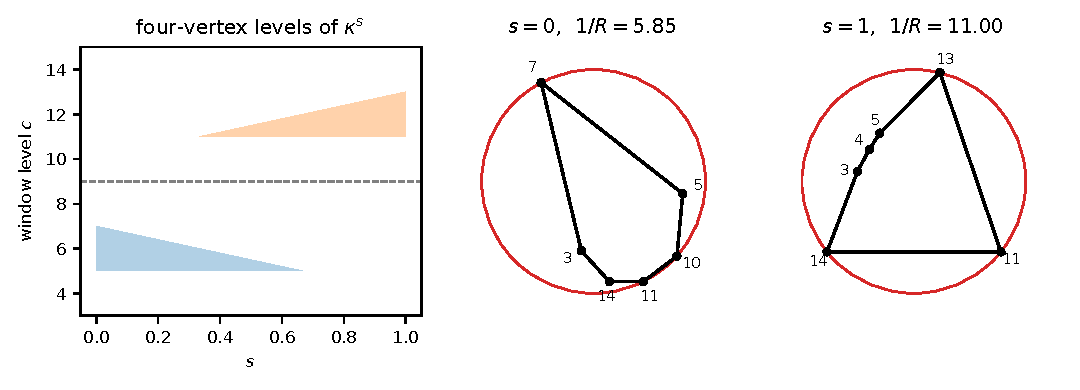
\includegraphics[width=0.8\textwidth]{tabachnikov/figures/hexagon.pdf}
\caption{Left: the levels of strict four-vertex windows of $\kappa^s$. Right:
realizing hexagons at $s=0$ and $s=1$ with their smallest enclosing circles.
The reciprocal enclosing radius is at most $7$ at $s=0$, at least $11$ at
$s=1$, and never $9$, so it cannot vary continuously.}
\label{fig:hexagon}
\end{figure}

A polygon $(P_i)_{i\in\Zn}$, not necessarily developed, \emph{realizes}
$\kappa$ if for every $i$ the circle through $P_{i-1},P_i,P_{i+1}$ has radius
$1/\kappa_i$.

\begin{theorem}\label{thm:hexagon}
There is no continuous map $s\mapsto P^s\in\C^6$, $s\in[0,1]$, such that each
$P^s$ is a coherent convex hexagon realizing $\kappa^s$.
\end{theorem}
% Lean: no_continuous_regular_hexagon_path
%       (Gluck/Discrete/GlobalContinuity/EnclosingCircleObstruction.lean); also
%       Gluck.Discrete.GlobalContinuity.no_continuous_tabachnikov_hexagon_path
%       for developed hexagons.

The invariant is the smallest enclosing circle. For a finite set $X$ of
points let $D(X)$ be its smallest enclosing closed disk and $R(X)$ its
radius; $D(X)$ exists and is unique, and $R$ is $1$-Lipschitz for the maximum
distance between labelled tuples, since enlarging a disk enclosing one tuple
by that distance encloses the other. The \emph{contacts} are the points of $X$
on $\partial D(X)$.
% Lean: enclosingRadius_lipschitz

\begin{lemma}\label{lem:contacts-determine}
$D(X)$ is also the smallest enclosing disk of its set of contacts.
\end{lemma}

\begin{proof}
Let $D(X)$ have center $O$ and radius $R$, and suppose a disk with center $O'$
and radius $R'<R$ contains every contact. For $O_t=(1-t)O+tO'$ and every
contact $x$,
\[
  |O_t-x|^2=(1-t)|O-x|^2+t|O'-x|^2-t(1-t)|O-O'|^2\le(1-t)R^2+tR'^2<R^2 ,
\]
and non-contacts satisfy $|O-x|<R$, hence $|O_t-x|<R$ for small $t>0$. Then a
disk of radius smaller than $R$ encloses $X$, a contradiction.
\end{proof}
% Lean: minimalEnclosingDiskR2_le_of_boundaryContactsInClosedDiskR2

In the next two lemmas $P$ is a coherent convex polygon with curvatures
$\kappa_i$, $D=D(P)$ has radius $R$, and $\omega_i$ is the circle through
$P_{i-1},P_i,P_{i+1}$, of radius $1/\kappa_i$.

\begin{lemma}\label{lem:contact-comparison}
If $P_i$ is a contact, then $\kappa_i\ge1/R$. If all contacts lie in
$\{P_{i-1},P_i,P_{i+1}\}$, then $\kappa_i\le1/R$.
\end{lemma}
% Lean: signedMengerProfile_inv_radius_le_of_minimal_boundary_of_cross_pos,
%       curvature_le_level_of_contacts_in_triple

\begin{proof}
Place $P_i$ at the origin with $D=\{z: |z|^2\le 2\langle O,z\rangle\}$,
$|O|=R$. The circle $\omega_i$ is $\{|z|^2=2\langle C,z\rangle\}$ with $|C|=1/\kappa_i$.
By coherence $C=aQ_-+bQ_+$ with $a,b\ge0$, where $Q_\pm=P_{i\pm1}$. Since
$Q_\pm\in\omega_i\cap D$,
\[
  |C|^2=a\langle C,Q_-\rangle+b\langle C,Q_+\rangle
  =\tfrac12\bigl(a|Q_-|^2+b|Q_+|^2\bigr)
  \le a\langle O,Q_-\rangle+b\langle O,Q_+\rangle=\langle O,C\rangle\le R\,|C| ,
\]
so $1/\kappa_i=|C|\le R$. For the second claim, the closed disk bounded by
$\omega_i$ contains all contacts, so its radius is at least $R$ by
Lemma~\ref{lem:contacts-determine}.
\end{proof}

\begin{lemma}\label{lem:containing}
If the disk bounded by $\omega_j$ contains every vertex, then
$\kappa_j\le\kappa_{j-1}$ and $\kappa_j\le\kappa_{j+1}$. If $P$ is not
inscribed in a circle, there are two vertices $j\ne j'$ with
$\omega_j\ne\omega_{j'}$ whose disks contain every vertex.
\end{lemma}
% Lean: containing_curvature_le_neighbors;
%       dahlbergE2Theorem6Lemma5ContainingDisks (Dahlberg 2008 manuscript, Lemma 5)

\begin{proof}
The circles $\omega_j$ and $\omega_{j+1}$ both pass through $A=P_j$ and
$B=P_{j+1}$, and by coherence both centers lie in the open half-plane $H$
bounded by the line $AB$ that contains the polygon. For circles through $A$
and $B$ with centers in $H$, the parts of their disks in $H$ increase strictly
with the radius. The vertex $P_{j+2}$ lies in $H$, on $\omega_{j+1}$ and in the
disk of $\omega_j$; if $\omega_{j+1}$ had the larger radius, $P_{j+2}$ would lie in
the open disk of $\omega_{j+1}$. Hence $1/\kappa_{j+1}\le1/\kappa_j$, and
symmetrically for $j-1$. The second statement is
Dahlberg's containing-circle lemma \cite{Dahlberg2008}, which applies to
strictly convex polygons not inscribed in a circle.
\end{proof}

\begin{proof}[Proof of Theorem~\ref{thm:hexagon}]
Suppose $P^s$ is such a family and put $c(s)=1/R(P^s)$, a continuous function.
Index the vertices $0,\dots,5$ as in~\eqref{eq:band}.

\emph{$c(s)\ne9$.} If $c(s)=9$, the contacts have $\kappa_i\ge9$ by
Lemma~\ref{lem:contact-comparison}, so they lie in $\{0,1,2\}$. The same
lemma at vertex $1$ gives $11=\kappa_1\le9$, which is absurd.

\emph{$c(0)\le7$.} If $c(0)>7$, the contacts lie in $\{0,1,2\}$, so
$c(0)\ge\kappa_1=11$. Then vertex $2$, with $\kappa_2=10$, is not a contact,
the contacts lie in $\{0,1\}\subset\{5,0,1\}$, and $c(0)\ge\kappa_0=14$. Now
the only possible contact is vertex $0$, and by
Lemma~\ref{lem:contacts-determine} the enclosing radius would be $0$.

\emph{$c(1)\ge11$.} Here $\kappa^1=(14,11,13,5,4,3)$. The hexagon is not
inscribed in a circle, since its profile is not constant. By
Lemma~\ref{lem:containing} there are two distinct vertices whose curvature
disks contain the polygon, and each is a weak local minimum of $\kappa^1$.
The only weak local minima are vertices $1$ and $5$, so vertex $1$ qualifies,
and $R\le1/\kappa_1=1/11$.

By the intermediate value theorem $c(s)=9$ for some $s$, a contradiction.
\end{proof}

The argument uses only continuity of the labelled vertices. Whether a global
continuous choice exists for $n=4$ or $n=5$ is left open.

\section{Circles tangent to consecutive sides}\label{sec:side-tangent}

There is a second discrete curvature attached to a convex polygon: the
reciprocal radius of the inward circle tangent to three consecutive
supporting lines. Wegner's four-edge theorem concerns these radii
\cite[Theorem~1]{Wegner1994}; see also \cite[Corollary~21.11]{Pak2010}. We give a converse as a companion to
Theorem~\ref{thm:main}. The construction below uses a tangential polygon and
positive edge scaling; it is independent of the four-length system used for
the main theorem.

\begin{definition}\label{def:side-tangent-circle}
Let $P_i$ be the vertices of a counterclockwise strictly convex polygon,
with outward unit normal $N_i$ on edge $[P_i,P_{i+1}]$.
The \emph{inward three-line circle at edge $i$} has center $C_i$ and radius
$r_i>0$ satisfying
\begin{equation}\label{eq:side-tangent-distances}
 \langle N_{i-1},P_i-C_i\rangle
 =\langle N_i,P_i-C_i\rangle
 =\langle N_{i+1},P_{i+1}-C_i\rangle=r_i.
\end{equation}
Its central contact is required to lie in the open edge $(P_i,P_{i+1})$.
The contacts on the two neighbouring supporting lines may lie on their
extensions. The circle need not be contained in the entire polygon.
\end{definition}
% Lean: Gluck.Discrete.SideTangent.ThreeLineCircle
% Lean: Gluck.Discrete.SideTangent.IsSideTangentRealization

\begin{figure}[htbp]
\centering
\figfile{side-tangent-circle}{0.52\textwidth}
\caption{The selected circle is tangent to three supporting lines, with
its central contact in the open edge. Here one neighbouring contact lies
beyond its edge. All coordinates, circle equations and contact parameters
in this example are checked with exact rational arithmetic.}
\label{fig:side-tangent-circle}
\end{figure}

Put $c_i=r_{i-1}-r_i$. By four cyclic sign changes we mean that there are
$i_1<i_2<i_3<i_4<i_1+n$ with
$c_{i_1}>0$, $c_{i_2}<0$, $c_{i_3}>0$ and $c_{i_4}<0$; zero differences are
retained but do not count as a sign. This formulation includes repeated
radii without a genericity assumption.

\begin{theorem}\label{thm:side-tangent-converse}
Let $n\ge4$ and let $r_i>0$ be a cyclic sequence. Suppose that $r$ is
constant or that $c_i=r_{i-1}-r_i$ has four cyclic sign changes. Then a
simple strictly convex polygon realizes $r_i$ as the radii of its inward
three-line circles. Each center and radius are uniquely determined by the
three equations~\eqref{eq:side-tangent-distances}, and every central contact
lies in its open edge.
\end{theorem}
% Lean: Gluck.Discrete.SideTangent.sideTangentConverse
% Lean: Gluck.Discrete.SideTangent.IsSideTangentRealization.tangent_sphere

The main ingredient is a balanced polygon circumscribed about the unit
circle. Its vertices, rather than the contact points, carry the coefficients.

\begin{lemma}\label{lem:side-tangent-balance}
Suppose $\sum_i c_i=0$ and $c$ has four cyclic sign changes. There is a
strictly convex polygon $Y_i$, circumscribed about the unit circle with each
contact in its open edge, such that $\sum_i c_iY_i=0$.
\end{lemma}
% Lean: Gluck.Discrete.SideTangent.exists_balanced_cyclicFan_of_dfv

\begin{proof}
Choose four alternating nonzero coefficients, and place their labels at
$(1,1),(-1,1),(-1,-1),(1,-1)$ in that order. Collapse all intervening labels
to the corresponding side contact of the square. All labels and their
coefficients remain present. Denote this limiting configuration by $X_i$,
and consider the finite rational field
\[
 G(a)=\sum_i\frac{c_i X_i}{1-\langle a,X_i\rangle}.
\]
For sufficiently small $\varepsilon>0$, all denominators are positive on
$D_\varepsilon=\{(x,y):|x|+|y|\le1-\varepsilon\}$. On its upper boundary arc
$y\ge |x|$, one of the two upper corner denominators equals $\varepsilon$.
If the alternating corner coefficients are $\alpha,-\beta,\gamma,-\delta$
with $\alpha,\beta,\gamma,\delta>0$, and the left and right contact
coefficients are $u,v$, then
\[
 \mathop{\rm Re}G(x,y)\ge
 \frac{\min(\alpha,\beta)}{\varepsilon}
       -\gamma-\delta-2|u|-2|v|>0.
\]
The upper and lower contact labels have zero horizontal contribution,
including near their poles. The corresponding bounds on the other three
arcs give, successively, $\mathop{\rm Im}G<0$ on the left,
$\mathop{\rm Re}G<0$ on the bottom and $\mathop{\rm Im}G>0$ on the right.
Thus the boundary field has winding number $-1$.

Now separate the repeated normals into small, strictly ordered clusters.
This produces a genuine tangential polygon $X_i^{\eta}$, with every edge
positive and every contact interior, converging to the labelled square as
$\eta\downarrow0$. Positivity of all denominators and the strict boundary
margins persist uniformly on the compact diamond. The perturbed field has
the same nonzero winding number and hence a zero $a$ in $D_\varepsilon$.
In particular $|a|<1$.

Set $\sigma=\sqrt{1-|a|^2}$ and
\[
 A=\sigma I+\frac{aa^{\mathsf T}}{1+\sigma},\qquad
 B_a(x)=\frac{Ax-a}{1-\langle a,x\rangle}.
\]
This projective transformation preserves the unit disk, its tangent lines,
and the cyclic order and open contacts of our polygon. All relevant
denominators are positive. Since $\sum_i c_i=0$,
\[
 \sum_i\frac{c_i}{1-\langle a,X_i^{\eta}\rangle}
 =\langle a,G(a)\rangle=0,
 \qquad
 \sum_i c_i B_a(X_i^{\eta})=A G(a)-a\langle a,G(a)\rangle=0.
\]
The vertices $Y_i=B_a(X_i^{\eta})$ have the required properties.
\end{proof}

\begin{lemma}\label{lem:side-tangent-scaling}
Let $Y_i$ be a counterclockwise strictly convex polygon circumscribed about the unit circle,
with its contacts in its open edges. If $r_i>0$ and
$\sum_i(r_{i-1}-r_i)Y_i=0$, the cyclic edge equations
\begin{equation}\label{eq:side-tangent-scaling}
 P_{i+1}-P_i=r_i(Y_{i+1}-Y_i)
\end{equation}
define a closed simple strictly convex polygon. Its inward three-line
circle at edge $i$ has center $C_i=P_i-r_iY_i$ and radius $r_i$.
\end{lemma}
% Lean: Gluck.Discrete.SideTangent.sum_scaled_edges
% Lean: Gluck.Discrete.SideTangent.strictSupport_of_positive_edge_scaling
% Lean: Gluck.Discrete.SideTangent.realizesSideTangent_of_scaledFan

\begin{proof}
Cyclic summation by parts gives
$\sum_i r_i(Y_{i+1}-Y_i)=\sum_i(r_{i-1}-r_i)Y_i=0$, so the edges close.
Positive scaling preserves their ordered directions and their total turn
of $2\pi$. For any fixed edge, the projections of the subsequent edges on
its left normal are first positive and then negative. Every intermediate
partial sum is positive, using closure for the second part. Hence every
nonincident vertex is strictly to its left. This gives strict support and
simplicity.

The outward normals satisfy
$\langle N_{i-1},Y_i\rangle=\langle N_i,Y_i\rangle=1$ and
$\langle N_{i+1},Y_{i+1}\rangle=1$. Substituting
$C_i=P_i-r_iY_i=P_{i+1}-r_iY_{i+1}$ gives all three
signed-distance equations. The central contact is the image of $N_i$ under
the positive homothety $x\mapsto C_i+r_ix$, and therefore lies in its open
edge. Adjacent normals are linearly independent. The first two equations
force any other center with radius $s$ to equal $P_i-sY_i$; the third then
gives $s=r_i$, since $\langle N_{i+1},Y_i\rangle<1$. Finally, unit normals
turn the signed-distance equations into actual circle tangency.
\end{proof}

\begin{figure}[tb]
\centering
\figfile{side-tangent-construction}{\textwidth}
\caption{A balanced polygon circumscribed about the unit circle (left) and
its positive edge scaling (right). The prescribed cyclic radii are
$(1,2,1,3/2,1,2,1,3/2)$. Closure, strict support and all eight circles are
verified exactly. The highlighted upper edge is the central edge of the
circle in Figure~\ref{fig:side-tangent-circle}.}
\label{fig:side-tangent-construction}
\end{figure}

\begin{proof}[Proof of Theorem~\ref{thm:side-tangent-converse}]
For nonconstant data, apply Lemma~\ref{lem:side-tangent-balance} to
$c_i=r_{i-1}-r_i$, whose sum is zero, and then
Lemma~\ref{lem:side-tangent-scaling}. For constant $r_i=r$, take a regular
polygon circumscribed about the unit circle and scale its edges by $r$.
\end{proof}

The forward implication is Wegner's four-edge theorem
\cite[Theorem~1]{Wegner1994}, whose convention already includes plateau
extrema. For the supporting-line circles of
Definition~\ref{def:side-tangent-circle}, we give a proof using the signed
affine-balance argument of \cite[Theorem~21.15]{Pak2010}, allowing zero
coefficients.

\begin{lemma}\label{lem:side-tangent-signs}
Let $Y_i$ be the cyclic vertices of a counterclockwise strictly convex polygon. If
$\sum_i c_i=0$ and $\sum_i c_iY_i=0$, then either every $c_i=0$ or the cyclic
coefficient sequence has at least four sign changes.
\end{lemma}
% Lean: Gluck.Discrete.SideTangent.zero_or_dfv_of_strict_affine_balance

\begin{proof}
A nonzero zero-sum sequence has both signs. If it has no four alternating
signs, it has one nonpositive block and one nonnegative block, with zeros
allowed in either. Choose a negative entry $c_a$ beginning the first block
and a positive entry $c_b$ beginning the second, using cyclic lifts
$a<b<a+n$. The chord $Y_aY_b$ has strictly negative signed area against
vertices in $(a,b)$ and strictly positive signed area against those in
$(b,a+n)$. Thus
\[
 c_i[Y_a,Y_b,Y_i]\ge0\quad\hbox{for every }i,
 \qquad \sum_i c_i[Y_a,Y_b,Y_i]=0,
\]
where $[A,B,C]$ is the signed determinant. The equality follows from the
zero mass and zero vector sum, since the determinant is affine in its third
argument. Every summand vanishes. Strict chord separation forces all
coefficients except $c_a,c_b$ to vanish. The two balance equations then give
$c_a(Y_a-Y_b)=0$, contradicting $c_a<0$ and distinctness of the vertices.
\end{proof}

\begin{corollary}\label{cor:side-tangent-iff}
Let $n\ge4$ and $r_i>0$. The sequence $r$ is realized by the inward
three-line circles of a simple strictly convex polygon, with their central
contacts in the open edges, if and only if $r$ is constant or its cyclic
differences $r_{i-1}-r_i$ have at least four sign changes.
\end{corollary}
% Lean: Gluck.Discrete.SideTangent.sideTangentForward
% Lean: Gluck.Discrete.SideTangent.realizesSideTangent_iff_admissible

\begin{proof}
Sufficiency is Theorem~\ref{thm:side-tangent-converse}. For necessity, start
from the actual polygon and its circles, and set
$Y_i=(P_i-C_i)/r_i$. The two incident normal equations give
$\langle N_{i-1},Y_i\rangle=\langle N_i,Y_i\rangle=1$.
These normals are linearly independent, because the polygon is strictly
convex. The circle at the preceding edge satisfies the same two normalized
equations at $P_i$, so it gives the same $Y_i$. Consequently
\[
 Y_{i+1}-Y_i=\frac{P_{i+1}-P_i}{r_i}.
\]
This is a closed positive edge scaling of the original polygon; the strict
support argument in Lemma~\ref{lem:side-tangent-scaling} therefore applies to
$Y$. Summation by parts gives
$\sum_i(r_{i-1}-r_i)Y_i=0$, and the differences themselves sum to zero.
Lemma~\ref{lem:side-tangent-signs} supplies four sign changes unless every
difference vanishes. In the latter case the cyclic radius sequence is constant.
\end{proof}

\section{Turning-angle curvature and the mixed-sign problem}\label{sec:discussion}

The choice of discrete curvature matters. Two elementary examples explain
why the results above neither extend to turning angles without further
hypotheses nor give a converse for arbitrary signed Menger profiles.

\subsection{Turning angles need not have four extrema}

If curvature is defined simply as the exterior turning angle, a strictly
convex polygon can have only one local maximum and one local minimum.

\begin{example}\label{ex:turning-angle}
Take the quadrilateral with counterclockwise vertices
\[
 A=(0,0),\qquad B=(3,0),\qquad C=(4,1),\qquad D=(0,2).
\]
It is strictly convex. Its exterior turns, in the same order, are
\[
 \theta_A=\frac{\pi}{2},\qquad
 \theta_B=\frac{\pi}{4},\qquad
 \theta_C=\frac{\pi}{2}+\arctan\frac35,\qquad
 \theta_D=\frac{\pi}{2}+\arctan\frac14.
\]
Thus $\theta_B<\theta_A<\theta_D<\theta_C$. Around the cycle
$A,B,C,D$, only $B$ is a local minimum and only $C$ is a local maximum.
All four readings are distinct, so plateau conventions do not affect the
example.
\end{example}

The construction is just a quadrilateral with unequal side lengths; there
is no limiting or degenerate configuration. It disproves the unrestricted
turning-angle version of the forward theorem. Additional assumptions can
restore such a statement: generic equilateral convex polygons with at least
four vertices satisfy an angle version of the discrete four-vertex theorem
\cite[Corollary~21.6]{Pak2010}.

\subsection{Four extrema do not suffice for mixed-sign Menger curvature}

For signed Menger curvature, the analogous difficulty concerns the
\emph{converse}. The strict four-vertex window alone does not guarantee
realizability once negative values are allowed.

\begin{example}\label{ex:mixed-sign}
For any $M,\varepsilon>0$, consider the cyclic profile
\begin{equation}\label{eq:mixed-counterexample}
 \kappa=(M,-\varepsilon,M,-\varepsilon).
\end{equation}
It has two strict maxima and two strict minima, and satisfies
$\DFV(\kappa,0)$: the two negative readings lie below zero and the two
positive readings above it. Nevertheless, no oriented simple quadrilateral
has this signed Menger profile.
\end{example}

\begin{proof}
For any counterclockwise simple polygon, let $\theta_i\in(-\pi,\pi)$ be its
principal exterior turns. They sum to $2\pi$. By~\eqref{eq:menger},
\[
 \kappa_i=\frac{2\sin\theta_i}{|P_{i+1}-P_{i-1}|},
\]
so $\kappa_i$ and $\theta_i$ have the same sign. There must therefore be at
least three positive curvature readings: with at most two positive turns,
\[
 2\pi=\sum_i\theta_i
 \le \sum_{\theta_i>0}\theta_i<2\pi,
\]
a contradiction. For a clockwise simple polygon the same argument with
signs reversed requires at least three negative readings. The profile
in~\eqref{eq:mixed-counterexample} has only two of each sign, so neither
orientation is possible.
\end{proof}

This obstruction is independent of coherence or local regularity. Making
$M$ arbitrarily large or $\varepsilon$ arbitrarily small does not remove it:
each individual positive turn is still less than $\pi$. Its moderate-arc
form is proved in \nolinkurl{Gluck/Discrete/Budget.lean}, by
\texttt{three\_le\_card\_pos\_of\_realizes} and
\texttt{killerProfile\_not\_realizes}. These Lean statements concern the
\texttt{RealizesR2} development model; the general polygon argument above
and Example~\ref{ex:turning-angle} are elementary arguments supplied here,
not separately formalized.

What additional conditions on a mixed-sign cyclic profile, beyond a strict
four-vertex window, characterize its realization as the signed Menger
curvature of a counterclockwise simple, locally regular polygon in the
sense of Dahlberg~\cite{Dahlberg2008}? The positive-support condition just
proved is necessary, but we do not claim it is sufficient. Thus the direct
mixed-sign extension is false, while finding the right strengthened
converse remains an open problem left by this work. Theorem~\ref{thm:main}
settles the positive case; a mixed-sign characterization would be a further
discrete counterpart of Dahlberg's smooth converse.

\subsection*{Acknowledgements}
The author would like to thank Aristotle, Claude, Codex, Deepseek for helpful
discussions. The proofs have been assisted with the use of AI but the author
takes full responsibility for their correctness.

\appendix
\section{Formal statements}\label{sec:lean}
\begingroup\raggedright\setlength{\parindent}{1.5em}

The main existence, continuity, and characterization results are proved in
Lean~4 (\texttt{v4.35.0}) with Mathlib in
\url{https://github.com/kejace/cd4vt} at version \texttt{\leancommit}, in the
library \texttt{Gluck}. Each displayed theorem depends only on the standard
axioms \texttt{propext}, \texttt{Classical.choice} and \texttt{Quot.sound}.
After \texttt{lake build}, the command
\texttt{lake env lean scripts/axioms.lean} prints these axioms for every
theorem below, using \texttt{\#print axioms}, for example
\begin{leancode}
#print axioms Gluck.Discrete.tabachnikov_converse_geometric
\end{leancode}
The paper sources name the Lean declarations behind the mathematical statements.

\subsection*{Theorem~\ref{thm:main}}
File \nolinkurl{Gluck/Discrete/TabachnikovConverse.lean}. Here
\texttt{vertexCircumradius v i} is the distance from \texttt{v i} to the
circumcenter of \texttt{v (i-1)}, \texttt{v i}, \texttt{v (i+1)}, and
\texttt{IsCoherentConvexPolygon} is simplicity, strict convexity and
coherence.
\begin{leancode}
theorem tabachnikov_converse_geometric [NeZero n]
    (hn : 4 ≤ n) {r : ZMod n → ℝ}
    (hr : ∀ i, 0 < r i) (hext : IsPlateauTwoMaxTwoMin r) :
    ∃ v : ZMod n → ℂ, IsCoherentConvexPolygon v ∧
      ∀ i, vertexCircumradius v i = r i
\end{leancode}

For this same polygon, the lemmas
\nolinkurl{IsCoherentConvexPolygon.signedMengerR2_eq_inv_of_radii} and
\nolinkurl{IsCoherentConvexPolygon.not_concyclic4_of_radius_ne}, in
\nolinkurl{Gluck/Discrete/TabachnikovCharacterization.lean}, give curvature
$1/r_i$ and exclude four consecutive concyclic vertices at each individual
pair with $r_i\ne r_{i+1}$. The original theorem
\texttt{tabachnikov\_converse}, with the combined conclusions, is retained.

\subsection*{Corollary~\ref{cor:iff}}
File \nolinkurl{Gluck/Discrete/TabachnikovCharacterization.lean}. The
hypotheses include positivity and nonconstancy, and the conclusion uses the
same distinct plateau runs as Theorem~\ref{thm:main}.
\begin{leancode}
theorem tabachnikov_radius_characterization [NeZero n]
    (hn : 4 ≤ n) {r : ZMod n → ℝ}
    (hr : ∀ i, 0 < r i) (hnc : ¬ ∃ c, ∀ i, r i = c) :
    (∃ v : ZMod n → ℂ, IsCoherentConvexPolygon v ∧
      ∀ i, vertexCircumradius v i = r i) ↔ IsPlateauTwoMaxTwoMin r
\end{leancode}

\subsection*{Theorem~\ref{thm:side-tangent-converse}}
File \nolinkurl{Gluck/Discrete/SideTangentConverse.lean}, namespace
\texttt{Gluck.Discrete.SideTangent}. The predicate
\texttt{SideTangentAdmissible r} means positive radii which are constant
or whose incoming-minus-outgoing differences have a strict four-sign window.
The predicate \texttt{RealizesSideTangent r} includes simplicity, strict
support, outward unit normals, all three signed-distance equations,
uniqueness of center and radius, and the open central contact.
\begin{leancode}
theorem sideTangentConverse [NeZero n] (hn : 4 ≤ n)
    (r : ZMod n → ℝ) (h : SideTangentAdmissible r) :
    RealizesSideTangent r
\end{leancode}
The same file proves \texttt{IsSideTangentRealization.tangent\_sphere}:
the sphere meets each of the three supporting lines in exactly its stated
contact point. Thus the linear equations imply metric circle tangency.

\subsection*{Corollary~\ref{cor:side-tangent-iff}}
File \nolinkurl{Gluck/Discrete/SideTangentForward.lean}, in the same
namespace and proof branch. The forward implication starts from an actual
\texttt{IsSideTangentRealization}; the balanced polygon and the necessary
sign condition are proved from it.
\begin{leancode}
theorem realizesSideTangent_iff_admissible [NeZero n]
    (hn : 4 ≤ n) (r : ZMod n → ℝ) :
    RealizesSideTangent r ↔ SideTangentAdmissible r
\end{leancode}
For positive nonconstant radii, \texttt{realizesSideTangent\_iff\_dfv}
removes the constant alternative and concludes
\texttt{DFV (radiusDifference r) 0} exactly.

\subsection*{Theorem~\ref{thm:local}}
File \nolinkurl{Gluck/Discrete/LocalContinuity.lean}. A
\texttt{LocalDiscreteRealizationFamily κ₀} is an open neighbourhood of
\texttt{κ₀} with a $C^1$ length map whose values are realizations and whose
vertex map is $C^1$. The strict window already implies nonconstancy and
$n\ge4$; neither needs to be a separate hypothesis.
\begin{leancode}
theorem localContinuousRealization_of_dfv [NeZero n]
    {κ₀ : ZMod n → ℝ} {c : ℝ}
    (hκ₀ : ∀ i, 0 < κ₀ i) (hdfv : DFV κ₀ c) :
    Nonempty (LocalDiscreteRealizationFamily κ₀)
\end{leancode}

\subsection*{Theorem~\ref{thm:hexagon}}
File \nolinkurl{Gluck/Discrete/GlobalContinuity/EnclosingCircleObstruction.lean},
where \texttt{bandProfile s} is $\kappa^s$ of~\eqref{eq:band}.
\begin{leancode}
theorem no_continuous_regular_hexagon_path :
    ¬ ∃ p : ℝ → (ZMod 6 → ℂ), ContinuousOn p (Set.Icc 0 1) ∧
      ∀ s ∈ Set.Icc (0 : ℝ) 1,
        IsSimplePolygon (p s) ∧ DahlbergRegular (p s) ∧
        SignedMengerProfile (p s) = bandProfile s
\end{leancode}
Here \texttt{DahlbergRegular} asks that at every vertex the circumcenter lie
in the closed vertex cone, with a collinear alternative when the middle
point lies between the others. The prescribed positive profile excludes
that alternative and already forces every consecutive triple to be positively
oriented. The function \texttt{SignedMengerProfile} is
$i\mapsto M(P_{i-1},P_i,P_{i+1})$. The orientation of a continuous path of
convex hexagons is constant, and complex conjugation reverses it; after
choosing counterclockwise orientation, a coherent convex realization of
$\kappa^s$ satisfies the three displayed conditions. Thus the formal statement
implies Theorem~\ref{thm:hexagon}.
\par\endgroup

\section{The acute orthogonal case}\label{sec:elimination}

We prove Proposition~\ref{prop:acute}. Let $L=\hat L(u,v)$ be as there and
suppose that $D\Ctrl(L)$ is not onto. All polynomial identities below were
verified by computer algebra and are checked in Lean.
% Lean: Gluck.Discrete.NativeOppositePure.fderiv_nativeLengthController_surjective_of_acute_orthogonal

\emph{Projective coordinates.} By Lemma~\ref{lem:core}(i),
$\cos\alpha_0=v\hat L_2$, $\cos\alpha_3=u\hat L_1$, $\cos\gamma_1=v\hat L_3$ and
$\cos\gamma_2=u\hat L_0$, hence
\begin{equation}\label{eq:tan}
  \tan\alpha_0\tan\gamma_2=\tan\alpha_3\tan\gamma_1=\frac{q}{uv}>1 .
\end{equation}
% Lean: Gluck.Discrete.NativeOppositePure.coreHalfLengths_angle_data,
%       coreHalfLengths_angles_acute, coreHalfLengths_tan, coreHalfLengths_tan_products,
%       coreHalfLengths_tan_product_gt_one
Put $x=\tan\alpha_0/\tan\gamma_1$, $y=1/(\tan\gamma_1\tan\gamma_2)$,
$w=1/\tan\gamma_2$ and $m=w^2$. By~\eqref{eq:tan}, $\tan\alpha_0=xw/y$,
$\tan\alpha_3=x/w$, $\tan\gamma_1=w/y$ and $\tan\gamma_2=1/w$. Since
$T<\pi/2$, $\tan\gamma_1\tan\gamma_2<1$, so $y>1$; and
$x/y=\tan\alpha_0\tan\gamma_2>1$, so $x>y>1$. With
$\lambda_*=\cos\alpha_0\cos\alpha_3/y>0$ one finds
\begin{equation}\label{eq:cos}
  \cos S=\lambda_*\,(y-x^2),\qquad \frac{\cos T}{q}=\lambda_*\,x\,(y-1);
\end{equation}
the first is $\cos S=\cos\alpha_0\cos\alpha_3(1-\tan\alpha_0\tan\alpha_3)$, and
the second uses $q\sin\alpha_3\cos\alpha_0=\cos\gamma_1\sin\gamma_2$, which
follows from the cosine relations above.
% Lean: Gluck.Discrete.NativeOppositePure.acute_projective_coordinates,
%       coreHalfLengths_normalized_cos

\emph{The equations.} By Lemma~\ref{lem:rank}, $AD=BC$. Put $a=A/2$, $b=C/2$
and $\tau=A/B$. Then $B=2a/\tau$ and $D=2b/\tau$, and since $0<p,l<1$ and
$t,h<q$, all of $A,B,C,D$ lie in $(0,1)$:
\begin{equation}\label{eq:ranges}
  0<a<\tfrac12,\quad 0<b<\tfrac12,\quad 2a<\tau,\quad 2b<\tau .
\end{equation}
% Lean: Gluck.Discrete.NativeOppositePure.incident_projective_parameters
Substituting~\eqref{eq:cos} into the second equation of~\eqref{eq:minors}
and dividing by $\lambda_*B$ gives
\begin{equation}\label{eq:affine}
  \mathcal A:=-(x+1)(x-y)(1+\tau)+2(x^2-y)b-2x(y-1)a=0 .
\end{equation}
% Lean: Gluck.Discrete.NativeOppositePure.projective_affine_of_incident_minor
Since $\tan\arcsin(c\sin z)=\varsigma_c(z)\tan z$, the four mixed arcsines
have tangents $(1-2a)\,xw/y$, $(1-2b)\,w/y$, $(1-2b/\tau)/w$ and
$(1-2a/\tau)\,x/w$. The equations $\varepsilon_1=0$ and $\varepsilon_3=0$ say
that four angles with nonzero cosines sum to $\pi$, and for such angles
$(\tan z_1\tan z_2-1)(\tan z_3+\tan z_4)=(\tan z_1+\tan z_2)(1-\tan z_3\tan z_4)$.
Clearing denominators gives
\begin{align}
  \mathcal E_1&:=y(x-m)\bigl(x(1-2a)+(1-2b)\bigr)
     -(x+1)\bigl(y^2-xm(1-2a)(1-2b)\bigr)=0,\label{eq:E1}\\
  \mathcal E_2&:=(xm-y^2)\,\tau\bigl(\tau-2b+x(\tau-2a)\bigr)
     -y(x+1)\bigl(m\tau^2-x(\tau-2b)(\tau-2a)\bigr)=0.\label{eq:E2}
\end{align}
% Lean: Gluck.Discrete.NativeOppositePure.tan_angleAtom_eq_slope_mul_tan,
%   tangent_turn_polynomial, first_projective_turn_polynomial,
%   second_projective_turn_polynomial, incidentProjectiveRankLoss_of_angles,
%   IncidentProjectiveRankLoss  (Lean names: P = x, Q = y, B = m, T = tau, r = a, k = b)
% Lean: Gluck.Discrete.NativeIncidentProjective.turnOne, turnTwo, affineRelation
So Proposition~\ref{prop:acute} follows from the next lemma.

\begin{lemma}\label{lem:elim}
There are no reals $x,y,m,a,b,\tau$ with $1<y<x$, $m>0$,
$a>0$, $0<b<\tfrac12$, $2a<\tau$ and $2b<\tau$ satisfying
\eqref{eq:affine}, \eqref{eq:E1} and~\eqref{eq:E2}.
\end{lemma}
% Lean: Gluck.Discrete.NativeIncidentProjective.not_projective_turn_solution
% Lean: Gluck.Discrete.NativeOppositePure.IncidentProjectiveRankLoss.false

\begin{proof}
Put
\[
  D_0=x(x+1)a-(x^2-y),\qquad N_0=(x+1)(x-y)+2x(y-1)a,\qquad
  \mathcal H=2bD_0+N_0 .
\]
\emph{Step 1: $\mathcal H=0$.} Write $\mathcal E_1=c_1m+d_1$ and
$\mathcal E_2=c_2m+d_2$; then $c_1d_2-d_1c_2=0$. Here
$c_1=-y(x(1-2a)+1-2b)+x(x+1)(1-2a)(1-2b)$,
$d_1=xy(x(1-2a)+1-2b)-(x+1)y^2$,
$c_2=x\tau(\tau-2b+x(\tau-2a))-y(x+1)\tau^2$ and
$d_2=-y^2\tau(\tau-2b+x(\tau-2a))+xy(x+1)(\tau-2b)(\tau-2a)$. Solving
\eqref{eq:affine} for $\tau$ (note $(x+1)(x-y)\ne0$) and substituting, one has
the identity of rational functions
\begin{equation}\label{eq:resultant}
  (x+1)(x-y)\,(c_1d_2-d_1c_2)\big|_{\tau=\tau(a,b)}
  =8xy\,(a-b)\,\bigl(b(x^2-y)+x^2a(y-1)\bigr)\,\mathcal H.
\end{equation}
% Lean: Gluck.Discrete.NativeIncidentProjective.elimination_identity (private),
%   projectiveH_eq_zero, projectiveH, projectiveD0, projectiveN
If $a=b$, then \eqref{eq:affine} reads $(x+1)(x-y)(2a-1-\tau)=0$, so
$\tau=2a-1<2a$, contradicting $\tau>2a$. Also $b(x^2-y)+x^2a(y-1)>0$. Hence
$\mathcal H=0$.

\emph{Step 2: two consequences.} The identities
\[
  (x+1)\bigl((x-y)\tau-2bxa\bigr)+\mathcal H+\mathcal A=0,
  \qquad
  D_0\,\mathcal E_1+(x+1)\,\mathcal C=c_H\,\mathcal H,
\]
with $c_H=2mx^2a-mx^2+2mxa-mx+my-xy$ and
$\mathcal C=m\,x\,\mathcal D(a)+y\,\mathcal P(a)$, where
\begin{align*}
  \mathcal P(a)&=2x^3a^2+(-3x^3+x^2y+x^2+xy)\,a+(x^3-x^2y-x^2+y^2),\\
  \mathcal D(a)&=2x(x+y-1)\,a^2+(-x^2-xy+3x-y)\,a+(y-x),
\end{align*}
give $(x-y)\tau=2bxa$ and $\mathcal C=0$.
% Lean: Gluck.Discrete.NativeIncidentProjective.projective_T_relation,
%   projective_polyC_eq_zero, polyA (= calP), polyD (= calD), polyC (= calC)

\emph{Step 3: a forced interval.} $N_0>0$, and $2bD_0=-N_0$ gives $D_0<0$.
From $(x-y)\tau=2bxa$ and $\tau>2b$ we get $a>(x-y)/x$. From $\mathcal H=0$,
$N_0+D_0=(1-2b)D_0<0$, and $N_0+D_0=x\bigl(a(x+2y-1)-(y-1)\bigr)$. Thus
\begin{equation}\label{eq:interval}
  a_-:=\frac{x-y}{x}<a<a_+:=\frac{y-1}{x+2y-1},
\end{equation}
% Lean: Gluck.Discrete.NativeIncidentProjective.projective_forced_interval
and in particular $a_-<a_+$, which is equivalent to $x^2-2y^2+y<0$.

\emph{Step 4: a sign obstruction.} $\mathcal P$ and $\mathcal D$ are convex
quadratics in $a$, so it suffices that each is negative at two points
bracketing~\eqref{eq:interval}. Direct evaluation gives
\begin{align*}
  \mathcal P(a_-)&=-xy(x-y), &
  \mathcal P\Bigl(\tfrac{x^2-y}{x(x+1)}\Bigr)&=-\frac{x(x+y)(x^2-2y+1)}{(x+1)^2},\\
  \mathcal D(a_-)&=\frac{(x-y)(x^2-xy-2y^2+y)}{x}, &
  \mathcal D(a_+)&=-\frac{y(x+y)(x^2-2y+1)}{(x+2y-1)^2}.
\end{align*}
Here $x^2-2y+1>2x-2y>0$, $x^2-xy-2y^2+y<x^2-2y^2+y<0$, and
$a_+<\frac{x^2-y}{x(x+1)}$, which after cross-multiplying is
$(x+y)(x^2-2y+1)>0$. So $\mathcal P(a)<0$ and $\mathcal D(a)<0$, hence
$\mathcal C<0$, contradicting $\mathcal C=0$.
\end{proof}
% Lean: Gluck.Discrete.NativeIncidentProjective.polyA_at_left, polyA_at_outer_right,
%   polyD_at_left, polyD_at_right, quadratic_neg_between (private),
%   polyA_neg_and_polyD_neg_of_interval, polyC_neg_of_interval


\bibliographystyle{amsplain}
\bibliography{tabachnikov/refs}

\end{document}
